\section{Annular comparison, the physical criterion, and mixed pins}
\label{an:section}

Throughout this section $J$ is fixed, $A_0=-\Delta_J/v_J^2$,
$k=\beta/v_J^2$, and $a=a(k)$ is the free-rectangle coefficient of
Theorem~\ref{st:free-rectangle-limit}.  A bare variance means the
variance of the real Gaussian with exactly the indicated quadratic
form.  All lattice pairings include the weights of the specified
discrete smear; in particular a probability cell smear has coefficients
equal to the reciprocal of its number of vertices.  Constants may
depend on $J,k$ and the fixed continuum geometry.  The limits in the
annular argument will always be taken in the following order:
\begin{equation}
 n\longrightarrow\infty,\qquad \ell\downarrow0,\qquad
 \lambda\longrightarrow\infty.
 \label{an:limit-order}
\end{equation}
Here $n^{-1}$ is the lattice spacing, $\ell$ the side of a mass cell,
and $\lambda$ its mass coefficient.  An error that vanishes in the
first two limits need not be uniform in $\lambda$.

The first part transfers the free-rectangle Gaussian coefficient to
Dirichlet domains and tori and identifies its positivity with physical
roughness, in Theorem~\ref{an:dirichlet-torus} and
Corollary~\ref{an:physical-criterion}.
The key step is Proposition~\ref{an:reach}, which makes the probability
that an exterior exploration reaches the test field vanish in the
stated order of limits.
The mixed-domain results that follow prepare Section~\ref{en:section};
their relative hard-pin comparisons remain useful when the pin
events themselves have small probability.

\subsection{A confining band and a sigma-finite cable representation}

Let $F$ be a fixed free square, let $D\Subset F$ be another square,
and let $g\in C_c^\infty(D)$.  Choose a closed polygonal annular
subband $K\Subset D\setminus\supp g$, of positive width, separating
$\supp g$ from $\partial D$.  Leave a positive gap on either side of
$K$.  Rational axis-parallel ring boundaries and lattice rounding
give the required geometry.  A regular partition of $K$ consists of
axis rectangles $d$ with sides comparable to $\ell$, with uniformly
bounded aspect ratios.  Write $|d|$ for their scaled counting areas and
\begin{equation}
 W_{\ell,\lambda}(h)=
 \exp\left\{-\frac\lambda2\sum_d |d|h_d^2\right\},
 \qquad S=(h,u),
 \label{an:band-weight}
\end{equation}
where $u$ is the uniform probability on $F_n$ and $h_d$ is the full
cell average.  In particular these averages are not projected to
mean zero.

There is a convenient canonical normalization of the free, unpinned
measure.  Choose the representative $h^0$ with $h^0_{x_0}=0$ of each
common-translation orbit, give these representatives their normalized
free Gaussian-lattice probability, and sum over
$h=h^0+2\pi m$, $m\in\Z$.  Denote the resulting sigma-finite measure
by $\mathcal P_n$.  Its definition is independent of the choice of
$x_0$: changing the representative only relabels the translation
sum on each orbit.  Define the probability
\begin{equation}
 \mathcal P_{n,W}=\widehat W\mathcal P_n,
 \qquad \widehat W=\frac{W}{\mathcal P_n(W)}.
 \label{an:band-probability}
\end{equation}
The denominator is finite and positive.  For example, conditionally
on the gradient representative, the band energy is a strictly
positive quadratic function of $2\pi m$; completing that square
proves finiteness of its translation sum, and Gaussian domination
controls the remaining mean-free linear functional.

\begin{lemma}[Band density and its limit]\label{an:band-density}
Suppose $a>0$.  For each fixed $\lambda>0$ and $1\le p<\infty$ there is
$\eta>0$ such that
\begin{equation}
 \limsup_{\ell\downarrow0}\limsup_{n\to\infty}
 \mathcal P_n(\widehat W^p e^{\eta S^2})<\infty.
 \label{an:density-moment}
\end{equation}
In the first two limits in \eqref{an:limit-order}, any finite list of
bounded piecewise continuous density smears under $\mathcal P_{n,W}$
converges, with all fixed moments, to the centered real Gaussian with
Neumann precision
\begin{equation}
 T_\lambda=\frac{-\Delta_F}{a}+\lambda 1_K.
 \label{an:band-precision}
\end{equation}
At each fixed partition, write
\[
 \mathcal T_{\ell,\lambda}(v,w)
 =a^{-1}\int_F\nabla v\cdot\nabla w
       +\lambda\sum_d|d|v_dw_d .
\]
The fixed-partition conclusion also includes any fixed finite list of
translation-invariant linear observations having uniformly bounded bare
variances and joint free convergence, with the band averages, to specified
continuous linear functionals on $H^1(F)$.  Their fixed-partition limiting
covariance is given by $\mathcal T_{\ell,\lambda}^{-1}$.  For a fixed such list, its
Laplace and fixed-moment limits are uniform when the coefficients of
linear combinations range over a fixed compact set.
In particular, for $X_n=(h,A_0g_n)$,
\begin{equation}
 \lim_{\ell\downarrow0}\lim_{n\to\infty}\Var_W X_n
       =a\int_F|\nabla g|^2.
 \label{an:band-saturation}
\end{equation}
The limiting fourth moments in this last statement are bounded
uniformly for $\lambda\ge\lambda_0>0$.
\end{lemma}

\begin{proof}
At a fixed partition, Theorem~\ref{st:free-rectangle-limit} and
Theorem~\ref{st:fractional-mean} give joint convergence of the
mean-free observations and of $S$ modulo $2\pi$, with the latter
uniform and independent.  Summing translations consequently
integrates the constant against $\dd c/(2\pi)$.  This assertion first
holds for continuous compactly supported functions of the actual
constant and a finite list of observations: periodize in the constant
and use the stated joint convergence.  To remove compact support,
put $\bar h_K=|K|^{-1}\sum_d|d|h_d$.  Jensen's Inequality gives
$\sum_d|d|h_d^2\ge |K|\bar h_K^2$, while
$S-\bar h_K$ is a mean-free smear of bounded bare variance.  Summing
the Gaussian translation tail and using Gaussian domination with a
slightly smaller negative coefficient gives uniform integrability
of every polynomial in the finitely many observations.  The same
argument allows a sufficiently small factor $e^{\eta S^2}$.
For an additional translation-invariant observation $X_n$ of uniformly
bounded bare variance, the one-dimensional Gaussian translation sum
also gives the direct bound
\[
 \sup_{h^0}\sum_{m\in\Z}W(h^0+2\pi m)<\infty
\]
at each fixed partition and strength.  Its weighted polynomial and
exponential tails are therefore controlled by the free subGaussian
tails of $X_n$.  The band normalizer has a positive limit at these fixed
parameters.  This proves the asserted extension to such observations;
the same bounds give equicontinuity in coefficients on compact sets.

For uniformity as the partition is refined, do the constant integral
first in the continuum.  The remaining penalty is $q$ times a
positive quadratic form in the mean-free Neumann field, for $W^q$.
It is the squared $L^2(K)$ norm of its cell projection with its
$K$-average subtracted.  Let $C_\ell$ be the covariance operator of
this projected field.  The nonzero Neumann eigenvalues of a square
are comparable to $m_1^2+m_2^2$.  Thus its inverse has square-summable
eigenvalues, and
\begin{equation}
 \sup_\ell\|C_\ell\|_{\mathrm{HS}}<\infty.
 \label{an:band-hs}
\end{equation}
If $t_j$ are the eigenvalues of $\lambda C_\ell$, the determinant
factor in $\mathcal P(W^p)/\mathcal P(W)^p$ has logarithm
\[
 \frac12\sum_j\{p\log(1+t_j)-\log(1+pt_j)\}.
\]
The linear terms cancel, and its absolute value is bounded by
$C_p\sum_jt_j^2$.  The explicit one-dimensional constant integrals
contribute bounded positive factors.  This proves the bound without
$e^{\eta S^2}$.  Neumann Poincar\'e's Inequality and the control of the
constant by $\bar h_K$ give
\[
 \|v\|_{L^2(F)}^2\le C_\lambda
 \left(a^{-1}\|\nabla v\|_2^2+
       \lambda\sum_d|d|v_d^2\right)
\]
uniformly under refinement.  The Gaussian covariance of $S$ under
the $p$-weighted measure is therefore uniformly bounded.  Its
one-dimensional Gaussian exponential integral proves
\eqref{an:density-moment} after decreasing $\eta$.  The fixed
partition lattice limit already proved transfers this bound in the
iterated-limsup sense asserted.

The cell projections converge strongly in $L^2(K)$.  The displayed
coercivity and weak $H^1$ compactness show that the corresponding
minimizers of $\frac12(v,Tv)-(f,v)$ converge to those for
$T_\lambda$.  Their energies converge as well, by using smooth
approximants as recovery sequences.  This proves convergence of the
inverse quadratic forms and hence of the finite Gaussian laws.
Uniform exponential moments just established permit moment
convergence.  Since $g$ vanishes near $K$ and $\partial F$,
$T_\lambda(ag)=-\Delta g$.  This proves
\eqref{an:band-saturation}.  Increasing $\lambda$ decreases the
continuum covariance, already finite at $\lambda_0$, so also gives
the final fourth-moment bound.
\end{proof}

The cable construction follows the metric-graph representation of
Gaussian fields \citep{Lupu2016,LupuWerner2018} and the Brownian
interpolation of the integer Gaussian field used by
\citet[Section~7]{AizenmanHarelPeledShapiro2022} to prove their
Proposition~7.1.
We give the edge-kernel disintegration and stopping argument explicitly
because the present unpinned measure is sigma-finite and the later
band penalty changes the sign law.

For the cable representation, give every retained unoriented bond
of conductance $c_e$ a unit-time independent Brownian bridge of
variance parameter $k/c_e$, conditional on its endpoint heights.
The unnormalized transition kernel is the edge weight times a
constant independent of the endpoints.  Call the bond open if the
bridge does not hit zero.  Given nonzero endpoints of the same sign,
its open probability is
$1-\exp(-2c_e|h_xh_y|/k)$; endpoints with different signs cannot be
joined by an open bond.  Splitting the bridge at the event of hitting
zero shows that the closed-edge weight does not couple endpoint
signs.  Consequently, conditionally on vertex magnitudes and the
open graph, the signs $\sigma_C$ of its nonzero components are
independent fair signs.  Zero singletons may be given independent
dummy signs.  Let $\omega=(|h|,\mathrm{open})$ and write the
height/open-state marginal as
\begin{equation}\label{an:sign-disintegration}
 \begin{aligned}
 \mathcal P_n(\dd h,\dd\mathrm{open})
     &=\nu_n(\dd\omega)\,\mathcal R_\omega(\dd\sigma),\\
 M_C(f)&=\sum_{x\in C}|h_x|f_x,\qquad
 m_C=M_C(u),\qquad Q_s=\sum_Cm_C^2.
 \end{aligned}
\end{equation}
This is a sigma-finite disintegration, rather than a probability
measure on $\omega$.  It can be constructed directly by summing the
finite sign configurations for every vector of magnitudes and every
edge state, with their nonnegative weights.  All calculations below
are first made for nonnegative integrands, so Tonelli's Theorem
applies before any finiteness is asserted.
To recover the full cable law, append the conditional bridge kernel
$\mathcal K_\omega(\dd\mathrm{cables}\mid\sigma)$, conditioned on these
endpoint values and edge states.  Thus the full law is
$\nu_n(\dd\omega)\mathcal R_\omega(\dd\sigma)
\mathcal K_\omega(\dd\mathrm{cables}\mid\sigma)$.
The sign-resampling statements below concern the height/open-state
marginal.  Before any stopping argument, its cluster integrals are
lifted to the full law by this kernel.

An exploration from a vertex reveals its value and reveals outgoing
bridges only until the next vertex or their first zero.  Continue at
every newly reached vertex.  The completed sigma-field records the
visited values, traversed segments, and the first-zero times and
locations on outgoing cut cables.  It does not reveal the remaining
segments.  The Brownian stopping property factors each unobserved
remainder as a transition kernel starting at zero.  The conditional
law of unvisited vertex heights is therefore a proper centered
Gaussian-lattice probability with zero boundary on the visited set
and conductances $c_e/t_e\ge c_e$ on cut remainders of length
$t_e\le1$.  Its unexplored sign clusters still have fair independent
signs.  A cluster sum can be disintegrated by declaring the least
vertex of each cluster to be its root.  The event that this root is
least is measurable at completion.  This counts every cluster once
and justifies conditional estimates for nonnegative intrinsic costs
depending only on that cluster's vertex magnitudes and open states.
These costs are measurable at completion, and their lifted integrals
may be conditioned on the realized cable segments and zero times.

\begin{lemma}[Path anchoring]\label{an:path-poincare}
Fix $r>0$.  After the completed exploration of a cluster of scaled
diameter at least $r$, the bare variance of the complement's
full-domain average, and of any fixed bounded density smear, is
bounded by a constant $V_r$.  If $\ell<r/C$ and $\mathcal D$ is any
collection of mass cells touched by that exploration, then
\begin{equation}
 \Var_{\mathrm{bare}}\left(
       \sum_{d\in\mathcal D}|d|b_d h_d^U\right)
    \le C\ell^2\sum_{d\in\mathcal D}|d|b_d^2.
 \label{an:local-path-bound}
\end{equation}
Here $U$ denotes unvisited vertices, and each average still uses the
full cell denominator.  The conclusion also holds when the starting
set is the entire exterior of $D$ and the exploration follows all
nonzero components meeting that set.  If a cell of side $\delta$ is
visited by a path arriving from distance at least a fixed multiple
of $\delta$, its remaining probability average has bare variance at
most $C$, independent of $\delta$.
\end{lemma}

\begin{proof}
Extend any variation on the unvisited vertices by zero on visited
vertices.  On a visited-to-unvisited nearest-neighbor edge the
posterior energy pays at least its original conductance times the
squared difference of this extension.  Thus the nearest-neighbor
energy of the zero extension is bounded by a fixed multiple of the
posterior energy.  The constant depends on $J$, which contains the
nearest-neighbor steps.

In a fixed-factor enlargement of a touched $\ell$-cell, stop a
visited path when it has first traveled distance $c\ell$ from its
initial point in that cell.  One coordinate projection spans
$c'\ell n$ levels.  Its jumps are bounded by $\max_{z\in J}|z|$;
there are therefore visited zeros on a fixed positive fraction of
these lattice levels.  Take a comparable enlarged rectangle with
$N\asymp\ell n$ rows and columns.  On each anchored row the
one-dimensional telescoping estimate gives
\[
 \sum_{x\text{ in row}}v_x^2
       \le C N^2\sum_{e\text{ in row}}(\nabla_ev)^2.
\]
Let $\bar v$ be the mean on the rectangle.  Since the anchored rows
contain a fixed fraction of its vertices,
\[
 N^2\bar v^2\le C\sum_{x\text{ in anchored rows}}v_x^2
                  +C\sum_x(v_x-\bar v)^2.
\]
The ordinary rectangle Poincar\'e Inequality controls the second sum
by $CN^2$ times the gradient energy.  Combining the two estimates
and dividing counting area by $n^2$ gives
\[
 n^{-2}\sum_{x\text{ in cell}}v_x^2
      \le C\ell^2\mathcal E_{\mathrm{post}}(v;
                                  \text{enlarged cell}).
\]
Enlargements have bounded overlap.  Cauchy--Schwarz for
$\sum |d|b_dv_d$ and the variational formula for inverse quadratic
forms prove \eqref{an:local-path-bound}.  With one fixed
$r$-sized anchored rectangle, the global Poincar\'e Inequality controls
the mean and energy on the whole connected square, proving the
$V_r$ assertion.  For an observation cell use the same proof at
scale $\delta$: its normalized density has squared $L^2$ norm
$O(\delta^{-2})$, canceling the $\delta^2$ in the local estimate.
For exterior exploration, the filled exterior supplies visited
zeros for the extension, and any path entering a touched interior
cell supplies the required segment.  No planarity of the $J$-bond
graph is used.
\end{proof}

\subsection{Cluster-mass tails, sign resampling, and tilt errors}

To use the exploration, we must control the cluster masses under the
band weight and the errors caused by resampling signs or changing the
posterior mean.  The next estimates provide these controls before the
reach argument compares the explored field with a centered pinned law.

For a mean-zero smear $f$ write
$\|f\|_{\mathrm{bare}}^2=k(f,A_{0,F}^{+}f)$, and for arbitrary $f$
put $f^0=f-u\sum_xf_x$.  The following bounds include the
sigma-finite normalization needed in the exploration argument.

\begin{lemma}[Finite bins and reinsertion]\label{an:reinsertion}
For $t\ge1$ and every fixed integer $p\ge1$,
\begin{align}
 \nu_n(Q_s\le4t^2)&\le C(1+t),\\
 \int_{Q_s\le4t^2}\left(\sum_CM_C(f)^2\right)^p\dd\nu_n
 &\le C_p(1+t)
       \left(t\left|\sum_xf_x\right|+
                    \|f^0\|_{\mathrm{bare}}\right)^{2p}.
 \label{an:bin-moments}
\end{align}
For mean-zero $f$, its squared-mass root also satisfies
\begin{equation}
 \nu_n\left(Q_s\le4t^2,
                \sum_CM_C(f)^2\ge z^2\right)
 \le C(1+t)\exp\left(-\frac{cz^2}{
                                  \|f\|_{\mathrm{bare}}^2}\right).
 \label{an:bin-tail}
\end{equation}
After exposing any cluster $C$ of diameter at least $r$, let $Q_U$
be the sum of squared complement cluster masses with the original
full-domain normalization.  For $0<\delta\le(4V_r)^{-1}$,
\begin{equation}
 \E(e^{\delta Q_U}\mid\mathcal F_C)\le3.
 \label{an:conditional-square-tail}
\end{equation}
Consequently, for every nonnegative intrinsic completed-cluster
cost $I(C)$ depending only on its vertex magnitudes and open states,
and $t\ge t_0(r)$,
\begin{equation}
 \int\sum_{C:\diam C\ge r} I(C)\ind_{m_C\le2t}\dd\nu_n
 \le 2\int\ind_{Q_s\le8t^2}
                 \sum_{C:\diam C\ge r}I(C)
                                      \ind_{m_C\le2t}\dd\nu_n.
 \label{an:reinsertion-bound}
\end{equation}
All these bounds are uniform in sufficiently fine meshes.
\end{lemma}

\begin{proof}
Given signless data, $\E_\sigma S^2=Q_s$.  Chebyshev's Inequality
gives $\Prob_\sigma(|S|\le Ct)\ge1-4/C^2$ on the bin.  For
$Y=(h,f)$, the Rademacher fourth-moment bound
$\E_\sigma Y^4\le3(\E_\sigma Y^2)^2$ and Paley--Zygmund give
fixed positive probability that
$|Y|\ge c(\sum_CM_C(f)^2)^{1/2}$.  Choose $C$ so the two events
intersect with a fixed positive probability.  On each gradient
orbit the number of translations satisfying $|S|\le Ct$ is at most
$C'(1+t)$.  A mean-zero $Y$ is translation invariant and has the
ordinary Gaussian upper tail by Lemma~\ref{st:finite-gaussian}.
This proves \eqref{an:bin-tail} and the first bound.  For general
$f$ use $Y=(h,f^0)+S\sum f$ on the same intersection, integrate the
tail, and obtain \eqref{an:bin-moments}.  Vanishing bare norm is
interpreted by continuity; then the corresponding mean-zero
functional vanishes identically.

Let $S_U$ be the signed complement mean.  Lemma~\ref{an:path-poincare}
and bare domination give
$\E(e^{zS_U}\mid\mathcal F_C)\le e^{V_rz^2/2}$.
Condition on the signless complement and use Jensen:
$Q_U^p\le\E_\sigma|S_U|^{2p}$.  Integrating the subGaussian tail
yields
\[
 \E(Q_U^p\mid\mathcal F_C)\le 2(2V_r)^pp!.
\]
Expansion of the exponential proves
$\E(e^{\delta Q_U}\mid\mathcal F_C)
 \le(1+2\delta V_r)/(1-2\delta V_r)\le3$.
For large enough $t_0(r)$ this implies
$\Prob(Q_U\le4t^2\mid\mathcal F_C)\ge1/2$.
Since $m_C^2\le4t^2$, this event gives $Q_s\le8t^2$.
Multiply by $I(C)\ind_{m_C\le2t}$, apply conditional expectation,
and sum using the least-root disintegration.  The argument applies
to extended nonnegative integrals, so does not presuppose the
finiteness it proves.
\end{proof}

\begin{lemma}[Damped tails and weighted moments]\label{an:weighted-moments}
For every $\eta>0$,
\begin{equation}
 \mathcal P_n\left(e^{-\eta S^2}
                      \ind_{t^2<Q_s\le4t^2}\right)
       \le C_\eta e^{-c_\eta t^2} \qquad(t\ge1).
 \label{an:damped-tail}
\end{equation}
If $a>0$, then at fixed $\lambda$ all fixed moments under
$\mathcal P_{n,W}$ of
squared cluster-mass sums and of signlessly selected partial signed
sums are bounded in the first two limits.  In particular, with
$D_\ell^2=1+\log(1/\ell)$ and any mass cell $d$,
\begin{equation}
 \E_W\left(\sum_CM_C(d)^2\right)^p
       +\E_W|d_*|^{2p}\le C_{p,\lambda}D_\ell^{2p},
 \label{an:cell-moments}
\end{equation}
where $d_*$ is any signed partial contribution selected from
signless data, with nonnegative coefficients bounded by the full
cell smear.  Fixed observation cells obey the same statement with
a fixed constant in place of $D_\ell$.
\end{lemma}

\begin{proof}
Choose a small fixed diameter threshold $r$ and a finite family of
separated probability box smears $p_j$ such that every cluster of
diameter less than $r$ misses at least one box.  If these small
clusters contribute at least $t^2/2$ to $Q_s$, assign each one a
missed box.  For that box $M_C(p_j-u)=-m_C$, so for some $j$ its
mean-zero squared-mass sum is at least $ct^2$.  Equation
\eqref{an:bin-tail} bounds this part of the bin by
$C(1+t)e^{-ct^2}$, even without the damping factor.

Otherwise the macroscopic clusters give the pointwise majorant
\[
 \ind_{t^2<Q_s\le4t^2}
 \le \sum_{C:\diam C\ge r}
     \frac{2m_C^2}{t^2}\ind_{m_C\le2t}\ind_{Q_s>t^2}.
\]
Expose each $C$.  Write $S=\sigma_Cm_C+S_U$.
If $m_C\ge t/2$, the events $|S_U|\le m_C/2$ and its complement
give
\[
 \E(e^{-\eta S^2}\mid\mathcal F_C)
 \le e^{-\eta m_C^2/4}+\Prob(|S_U|>m_C/2\mid\mathcal F_C)
 \le Ce^{-ct^2}.
\]
If $m_C<t/2$, the condition $Q_s>t^2$ implies
$Q_U>3t^2/4$, whose conditional probability has the same bound by
\eqref{an:conditional-square-tail}.  The remaining intrinsic sum
$\sum (m_C^2/t^2)\ind_{m_C\le2t}$ is finite after
\eqref{an:reinsertion-bound}; indeed on its reinserted bin its
pointwise value is bounded by a constant and the bin has mass
$O(1+t)$.  Absorbing this factor proves \eqref{an:damped-tail}.

To transfer moments, let $H$ be a squared-mass root or a selected
signed sum, and let $A_t$ be a dyadic bin for $Q_s$.  Conditional
Khintchine bounds followed by \eqref{an:bin-moments} give
$\mathcal P_n(|H|^{2p}\ind_{A_t})\le P_p(t)D^{2p}$, for a
polynomial $P_p$ and the appropriate bare-cost scale $D$.
H\"older's Inequality with exponents $4,4,2$ gives
\begin{align*}
 \mathcal P_n(\widehat W|H|^p\ind_{A_t})
 &\le
 \mathcal P_n(\widehat W^4e^{\eta S^2})^{1/4}
 \mathcal P_n(e^{-\eta S^2}\ind_{A_t})^{1/4}
 \mathcal P_n(|H|^{2p}\ind_{A_t})^{1/2}.
\end{align*}
The exponential factors cancel exactly in this application.
Equations~\eqref{an:density-moment} and \eqref{an:damped-tail}
make the dyadic sum finite and its tail uniformly small.  The
lowest bin is handled directly by \eqref{an:bin-moments}.

For completeness, the bare variance of $h_d-S$ is
$O(1+\log(1/\ell))$.  Cut and compare to a fixed containing square
using nearest-neighbor edges.  In its discrete Neumann cosine
basis the rescaled coefficients of a probability $\ell$-cell
smear are bounded.  Summing inverse eigenvalues up to frequency
$\ell^{-1}$ costs $C\log(1/\ell)$.  Above that frequency,
Parseval and the bound $\|d-u\|_2^2=O(\ell^{-2})$ give a bounded
remainder.  This proves \eqref{an:cell-moments}.  The same argument
works with an independent auxiliary fair-sign sample: exchanging
the old and new samples preserves the base measure, so the density
moment estimate is unchanged.
\end{proof}

\begin{lemma}[Asymptotically fair macroscopic signs]\label{an:resampling}
Suppose $a>0$, and fix $r>0$ and $\lambda>0$.  In the height/open-state
marginal, jointly replacing the signs of all
clusters of diameter at least $r$ by fresh independent fair signs
changes the band law by a total variation error tending to zero as
$n\to\infty$ and then $\ell\downarrow0$.  The contribution of
clusters of diameter below $r$ to any fixed bounded density smear
tends to zero in every fixed moment when $r\downarrow0$ after
these two limits.  For nonnegative such smears $f,p$,
\begin{equation}
 \limsup_{\ell\downarrow0}\limsup_{n\to\infty}
 \E_W\sum_{C:\diam C\ge r}M_C(f)M_C(p)
      \le (f,T_\lambda^{-1}p).
 \label{an:cross-cluster}
\end{equation}
All fixed moments of $\sum_{\diam C\ge r}M_C(f)^2$ have limiting
upper bounds uniform for $\lambda\ge\lambda_0>0$.
\end{lemma}

\begin{proof}
On $Q_s\le t^2$, expand the difference of the two quadratic mass
energies in the original and resampled signs.  Orthogonality of
Rademacher monomials bounds its squared base integral by
\begin{equation}
 C\lambda^2\int\ind_{Q_s\le t^2}
 \sum_{C:\diam C\ge r}\sum_{C'\ne C}
       \left(\sum_d|d|M_C(d)M_{C'}(d)\right)^2\dd\nu_n.
 \label{an:resampling-square}
\end{equation}
Expose $C$, retain the intrinsic condition $m_C\le t$, and drop
the complement truncation.  The inner sum, after its fair signs
are averaged, is the conditional second moment of
$\sum_d|d|M_C(d)h_d^U$.  Equation~\eqref{an:local-path-bound}
bounds it by $C\ell^2\sum_d|d|M_C(d)^2$.  Reinsert
$Q_s\le C(1+t^2)$ using Lemma~\ref{an:reinsertion}, and then use
\eqref{an:bin-moments}.  The result is
\begin{equation}
 \mathcal P_n\left(\ind_{Q_s\le t^2}
          |\log W(\sigma')-\log W(\sigma)|^2\right)
        \le C_{\lambda,t,r}\ell^2D_\ell^2+o_n(1).
 \label{an:resampling-rate}
\end{equation}
The bin has finite base mass.  Equation~\eqref{an:density-moment}
gives uniform $L^p$ bounds for both normalized densities there.
Split where the logarithmic difference is larger than a fixed
$\delta$; on that set use H\"older and
\eqref{an:resampling-rate}, and on its complement use
$|e^x-e^y|\le(e^\delta-1)(e^x+e^y)$.
First take the two mesh limits, then $\delta\downarrow0$.
Lemma~\ref{an:weighted-moments} removes the bin cutoff.  This
proves total variation convergence, also against functions with
the moment bounds of that lemma.

Partition $F$ into $r$-cells.  A cluster of diameter below $r$
meets only a bounded number of neighboring cells.  For a bounded
density $f$, Cauchy--Schwarz over those cells bounds its squared
mass contribution by $C\|f\|_\infty^2r^4$ times the sum of the
cell squared-mass contributions.  There are $O(r^{-2})$ cells.
Equation~\eqref{an:bin-moments} consequently gives, on a fixed
bin, signed second moment at most
$C_t\|f\|_\infty^2r^2(1+\log(1/r))$.
Higher fixed moments are bounded there.  Interpolation, the
H\"older transfer in Lemma~\ref{an:weighted-moments}, and its tail
truncation prove the asserted vanishing in moments.

Resample signs first at a threshold smaller than $r$.  The fair
second moment of the macroscopic signed contributions is their
squared-mass sum, and all terms for nonnegative smears are
nonnegative.  Remove the still smaller clusters by the preceding
bound and apply Lemma~\ref{an:band-density} to the full smears.
This proves \eqref{an:cross-cluster}.  Jensen in the signs gives
$(\sum M_C(f)^2)^p\le\E_\sigma|\sum\sigma_CM_C(f)|^{2p}$;
the same resampling and small-cluster argument bounds its limit
by the Gaussian $2p$-moment.  The covariance decreases with
$\lambda$ and is finite at $\lambda_0$, giving the stated
uniformity.
\end{proof}

\begin{lemma}[Finite tilt and size-bias inequalities]
Let $\mu$ be any proper centered Gaussian-lattice probability.\label{an:tilt}
Suppose the bare variances of real linear tests $L,X$ are at most
$\eps^2,V$, respectively, where $\eps\ge0$ and $V>0$, and put
$\dd\mu_L=e^L\dd\mu/\mu(e^L)$.  Then, for every $z\ge0$,
\begin{align}
 |\E_LX|&\le2\sqrt V\,\eps,\\
 \mu_L\{|X|\ge\sqrt V(2\eps+z)\}&\le2e^{-z^2/2},\\
 |\E_LX^2-\E X^2|+|\Var_LX-\Var X|
       &\le CV\eps(1+\eps).
 \label{an:tilt-bounds}
\end{align}
The mean and second-moment/variance estimates also hold for $V=0$,
when $X=0$ almost surely; the displayed closed-tail inequality is
asserted only for $V>0$.
For every inversion-symmetric event $E$ of positive probability,
\begin{equation}
 \mu_L(E)\ge e^{-\eps^2/2}\mu(E).
 \label{an:relative-tilt}
\end{equation}
For any two real linear tests $X,Y$ under $\mu$,
\begin{equation}
 \E[X^2|Y|]\ge\E X^2\,\E|Y|.
 \label{an:size-bias}
\end{equation}
\end{lemma}

\begin{proof}
Symmetry and bare domination give $1\le\mu(e^L)$ and
$\mu(e^{L+tX})\le\exp((\eps+|t|\sqrt V)^2/2)$.
Convexity applied at $t=\pm\eps/\sqrt V$ proves the mean bound;
if $\eps=0$, then $L=0$ almost surely and the mean bound follows
from centeredness.  For $V>0$ and $z\ge0$, Chernoff with this same
bound proves the displayed tail.  The case $V=0$ gives $X=0$
almost surely and hence the non-tail estimates directly.
If $\eps\le1$, then
\[
 \mu((e^L-1)^2)\le e^{2\eps^2}-1\le C\eps^2.
\]
Cauchy--Schwarz, the bare fourth-moment bound, and the denominator
at least one give the second-moment error $CV\eps$.  Subtracting
the squared mean gives the variance error.  For $\eps\ge1$ the
tail bound controls the two second moments by $CV(1+\eps)^2$,
which proves \eqref{an:tilt-bounds}.  Conditional symmetry on $E$
gives $\mu(e^L\mid E)=\mu(\cosh L\mid E)\ge1$, proving
\eqref{an:relative-tilt}.

For the final assertion let $\phi(t)=\E\cos(tY)>0$.
The minimal log Hessian of the positive characteristic function
from Lemma~\ref{st:finite-gaussian}, applied in the $X$ direction
at frequency $tY$, gives
\[
 \E[X^2\cos(tY)]\le \E X^2\,\phi(t)
                    -\frac{(\E[X\sin(tY)])^2}{\phi(t)}.
\]
Subtract from the equality at $t=0$ and integrate the weaker
inequality against $2\dd t/(\pi t^2)$ on $(0,\infty)$.
The identity $|y|=(2/\pi)\int_0^\infty(1-\cos ty)t^{-2}\dd t$
and Tonelli prove \eqref{an:size-bias}.  The bias $|Y|$ preserves
inversion symmetry, so its mean for $X$ is zero.
\end{proof}

When an exploration is performed under the band law, write
$h_d=d_*+h_d^U$.  Relative to the centered posterior with the
restricted band quadratic form, the remaining tilt is
$L=-\lambda\sum_d|d|d_*h_d^U$.  Equation
\eqref{an:local-path-bound} gives
\begin{equation}
 \eps^2\le C\lambda^2\ell^2\sum_d|d|d_*^2.
 \label{an:exterior-tilt}
\end{equation}
For a single exposed macroscopic cluster define $\eps_C$ by the
same bound with $|d_*|=M_C(d)$.  Put
$E_2=\sum_{\diam C\ge r}\eps_C^2$.  If $a>0$, Equation
\eqref{an:cell-moments} and weighted Jensen give, for each fixed
$p$ and $\lambda$,
\begin{equation}
 \E_W\eps^{2p}+\E_WE_2^p
       \le C_{p,\lambda,r}\ell^{2p}D_\ell^{2p}+o_n(1).
 \label{an:tilt-moments}
\end{equation}
For two fixed observation cells $B,i$, write
$Q_B=\sum_{\diam C\ge r}M_C(B)^2$ and define $Q_i$ likewise.
The exact summation bound needed below is
\begin{align}
 &\sum_{\diam C\ge r}M_C(B)\eps_C(1+\eps_C)(1+M_C(i))
 \notag\\
 &\hspace{1cm}\le
 \sqrt{Q_B}(1+\sqrt{Q_i})(\sqrt{E_2}+E_2).
 \label{an:summed-tilt}
\end{align}
Indeed use Cauchy--Schwarz for the sum of $M_C(B)\eps_C$,
and bound $\sup_C\eps_C$ and $\sup_CM_C(i)$ by the square roots
of their respective squared sums.  For $a>0$, H\"older and the moment bounds
show that the expectation in \eqref{an:summed-tilt} is
$O_{\lambda,r}(\ell D_\ell+\ell^2D_\ell^2)$ in the mesh limit.
There is no factor counting microscopic clusters.

\subsection{Stopping the exploration and transferring the field}

\begin{figure}[t]
\centering
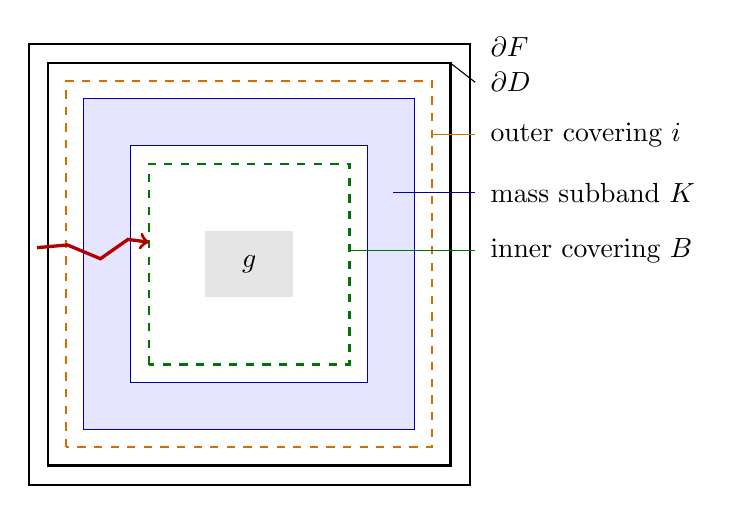
\begin{tikzpicture}[scale=.70]
 \fill[blue!10,even odd rule] (-3,-3) rectangle (3,3)
                           (-2.15,-2.15) rectangle (2.15,2.15);
 \draw[thick] (-4,-4) rectangle (4,4);
 \draw[thick] (-3.65,-3.65) rectangle (3.65,3.65);
 \draw[blue!65!black] (-3,-3) rectangle (3,3);
 \draw[blue!65!black] (-2.15,-2.15) rectangle (2.15,2.15);
 \draw[dashed,orange!85!black,thick] (-3.32,-3.32) rectangle (3.32,3.32);
 \draw[dashed,green!45!black,thick] (-1.82,-1.82) rectangle (1.82,1.82);
 \fill[gray!20] (-.8,-.6) rectangle (.8,.6);
 \node at (0,0) {$\supp g$};
 \node[anchor=west] at (4.2,3.95) {$\partial F$};
 \node[anchor=west] at (4.2,3.30) {$\partial D$};
 \draw (4.1,3.30)--(3.65,3.65);
 \node[anchor=west] at (4.2,2.35) {outer covering $i$};
 \draw[orange!85!black] (4.1,2.35)--(3.32,2.35);
 \node[anchor=west] at (4.2,1.30) {mass subband $K$};
 \draw[blue!65!black] (4.1,1.30)--(2.60,1.30);
 \node[anchor=west] at (4.2,.25) {inner covering $B$};
 \draw[green!45!black] (4.1,.25)--(1.82,.25);
 \draw[->,very thick,red!70!black]
       (-3.85,.3)--(-3.30,.35)--(-2.7,.1)--(-2.2,.45)--(-1.82,.4);
\end{tikzpicture}
\caption{The annular comparison, schematically.  The coverings
are finite unions of small cells around the dashed rings.  They
have positive clearance from the mass subband, the test support,
and $\partial D$.  An exploration reaching the test support from
$F\setminus D$ must pass both coverings.  The drawing does not
restrict the finite-range paths to nearest-neighbor paths.}
\label{an:band-figure}
\end{figure}

\begin{proposition}[Vanishing reach]\label{an:reach}
Suppose $a>0$.  Under the band law, explore all components meeting $F_n\setminus
D_n$.  The probability that any visited vertex is in a fixed
neighborhood of $\supp g$ tends to zero in
\eqref{an:limit-order}.  The same conclusion holds for an
exploration starting from a fixed positive-area region on one
side of a separating positive-width band and reaching a fixed
closed region on its other side, provided the closure of the starting
region and the target have fixed positive clearance from the band.
The two gaps admit the mass-free covering families used below, with
all clearances fixed before the lattice and band limits.
\end{proposition}

\begin{proof}
Choose finite coverings by small observation squares $B$ of an
inner ring and by squares $i$ of an outer ring, leaving the
clearances shown in Figure~\ref{an:band-figure}.  Use slightly
overlapping enlarged squares so every path crossing the rings
hits the coverings also after lattice rounding.  The maximum
scaled jump tends to zero, so a path from the starting set to the
target must meet both coverings, in order.

Let $C_0$ be the uniform bare variance bound for the remaining
average in a cell reached by a path from afar, from
Lemma~\ref{an:path-poincare}.  The cell radii can be chosen so
small that their continuum prior variances under $T_\lambda^{-1}$
are at least $C_0+2c_0$ for some $c_0>0$, uniformly over
$\lambda>0$.  To see this directly, center a truncated logarithm
at the cell and cut it off inside a fixed surrounding ball
disjoint from the mass.  Its mean over a radius-$\delta$ cell is
$c\log(1/\delta)+O(1)$, while its gradient energy is
$c'\log(1/\delta)+O(1)$.  The inverse variational principle
therefore makes the cell-average variance grow at least as
$c''a\log(1/\delta)$.  This trial pays no mass term.  Fix the
coverings at this point.  Lemma~\ref{an:band-density} gives the
same strict deficit $c_0$ for fine $\ell,n$ at each fixed
$\lambda$.

Write the average at $B$ after exterior exploration as
$h_B=e_B+u_B$, its exposed and unexposed contributions.  On
omitting the linear tilt, the conditional form is obtained from
the prior form by zero-pinning visited vertices and tightening
the cable remainders.  The partial average $u_B$ is precisely
the original full test after those zero pins.  Thus its centered
variance $w_B$ is at most the full prior variance $v_B$ by
Lemma~\ref{st:finite-gaussian}, and on a visit to $B$ it is at
most $v_B-c_0$ by the local bound.  Equations
\eqref{an:tilt-bounds} and \eqref{an:tilt-moments} show that
restoring the tilt changes the conditional second moment, and
the cross term with $e_B$, by $o(1)$ after averaging.  The needed
moments of $e_B$ follow from Lemma~\ref{an:weighted-moments}.
The prior identity $\E h_B^2=v_B$ consequently implies
\[
 c_0\Prob_W(B\text{ reached})\le\E_We_B^2+o(1).
\]
Every cluster contributing to $e_B$ is macroscopic, with a
threshold fixed by its distance from the starting set.  Sign
resampling, including the same signless selection of exterior
clusters, converts its second moment to the squared-mass sum:
\begin{equation}
 c_0\Prob_W(B\text{ reached})
 \le\E_W\sum_{C\text{ meeting the starting set}}M_C(B)^2+o(1).
 \label{an:exterior-deficit}
\end{equation}

A second deficit bounds this right side.  For each $x\in B$
with $\E_W|h_x|>0$, bias the prior by $|h_x|$ and explore only
the cluster of $x$.  Its pre-exploration variance for $h_i$ is
at least $v_i$ by \eqref{an:size-bias}.  The bias is measurable
at completed exploration and hence cancels from the conditional
law of the complement.  Its centered remaining variance is at
most $v_i$, and is at most $v_i-c_0$ if the cluster visits $i$.
Its exposed average has absolute value $M_{C(x)}(i)$.
Apply total second moment in this biased law, multiply by
$\E_W|h_x|$ and the averaging weight of $x$ in $B$, and sum in
$x$.  The terms without a visit or a tilt cancel in the
comparison with $v_i$.  Clusters causing a tilt must reach the
mass cells, and clusters contributing at $i$ must reach $i$;
both are macroscopic because all three regions have positive
separation.  Their remaining errors are bounded by a constant
times the expectation in \eqref{an:summed-tilt}, which tends
to zero.  A point with $\E_W|h_x|=0$ contributes zero directly.
The result is the exact weighted deficit
\begin{equation}
 c_0\E_W\sum_{C:C\cap i\ne\varnothing}M_C(B)
       \le\E_W\sum_CM_C(B)M_C(i)^2+o(1).
 \label{an:biased-deficit}
\end{equation}
In particular no estimate on an unsigned sum over all
microscopic clusters has been used.

The inverse forms $T_\lambda^{-1}$ decrease as
$\lambda\to\infty$ to the form inverse with every function
zero almost everywhere on $K$.  Indeed bounded energies give
weak $H^1$ compactness and $\int_Kv^2\to0$; the variational
principle gives both the limit and recovery by functions already
zero there.  This hard band separates the inner and outer
regions, so its inverse has zero cross quadratic form for
smears on opposite sides.  Equation~\eqref{an:cross-cluster}
therefore makes $\E\sum_CM_C(B)M_C(i)$ tend to zero after
\eqref{an:limit-order}.  Truncate first at
$\max_CM_C(i)\le M$.  On this event the right side of
\eqref{an:biased-deficit} is at most $M$ times this vanishing
cross sum.  Its tail tends to zero uniformly as $M\to\infty$:
\[
 \sum_CM_C(B)M_C(i)^2\le\sqrt{Q_B}\,Q_i,
\]
and Lemma~\ref{an:resampling} gives arbitrarily high uniform
moments after the first two limits.  Thus
$\E\sum_{C\cap i\ne\varnothing}M_C(B)\to0$.

Every exterior-connected cluster meeting $B$ must visit some
outer covering cell $i$.  On $\max_CM_C(B)\le M$ its
contribution to \eqref{an:exterior-deficit} is at most $M$ times
the sum of the just estimated first-mass quantities.  The
remaining tail is again controlled by the uniform moments of
$Q_B$.  Send $M\to\infty$ after the three limits.  Each $B$ is
reached with probability tending to zero, and their finite
cover gives the assertion.  The proof for a different starting
region only replaces the filled exterior by that region; the
path anchoring and the two separated coverings have exactly the
same hypotheses.
\end{proof}

\begin{theorem}[Dirichlet and torus transfer]\label{an:dirichlet-torus}
For $a(k)>0$, the centered, unprojected zero-Dirichlet height law
on every fixed square converges, in smooth density observations
and their Laplace transforms, to the real zero-Dirichlet GFF of
covariance $a(k)(-\Delta_D)^{-1}$.  For growing square tori, at
every $k>0$ the mean-subtracted height field converges to the
mean-zero torus GFF with covariance $a(k)(-\Delta_{\T^2})^{-1}$,
where $a=0$ denotes the zero distribution.  Convergence holds
along every sequence of increasing integer side lengths and in
$H^{-3}(\T^2)$.  For smooth mean-zero $f$,
\begin{equation}
 \lim_{n\to\infty}\log\E e^{H_n(f)}
     =\frac{a(k)}2(f,(-\Delta_{\T^2})^{-1}f).
 \label{an:torus-laplace}
\end{equation}
On the positive branch the uniquely determined temperature
coefficient in Equation~\eqref{main:coefficient-convention} is
\begin{equation}
 \beff(J,\beta)=v_J^2a(\beta/v_J^2).
 \label{an:effective-temperature}
\end{equation}
\end{theorem}

\begin{proof}
Consider $X_n=(h,A_0g_n)$ in the free square with the band.
On the success event of Proposition~\ref{an:reach}, the exposed
contribution to $X_n$ is zero.  Its centered conditional
variance is at most its massless zero-Dirichlet variance in
$D_n$: the centered posterior has zeros on the whole exterior,
possibly further pins and tightened edges, and the remaining
positive band precision.  Drop the latter extra conditions
using Lemma~\ref{st:finite-gaussian}.  The linear-tilt error
vanishes by \eqref{an:tilt-bounds} and
\eqref{an:tilt-moments}.  On failure, Cauchy--Schwarz bounds
$\E_W[X_n^2\ind_{\mathrm{failure}}]$ by its fourth-moment
root times the square root of the failure probability.
Lemma~\ref{an:band-density} bounds this fourth moment uniformly
after the first two limits and toward the last limit.  Hence
\eqref{an:band-saturation} implies
\begin{equation}
 \liminf_{n\to\infty}\Var_D(h,A_0g_n)
      \ge a\int_D|\nabla g|^2.
 \label{an:dirichlet-lower}
\end{equation}
This is valid along every subsequence of lattice sizes: one
uses that subsequence in the band argument before the other
limits.  Free-square cutting gives the opposite bound, with
the same gradient energy, for the zero-Dirichlet law.  Its
logarithmic moment generating function has the covariance
quadratic lower bound of Lemma~\ref{st:finite-gaussian}.
The matching upper bound follows by cutting into cells of
relative side $r$, Taylor-expanding their centered
subGaussian logarithmic moment generating functions to second
order, and summing the $O(r^3)$ remainder over $O(r^{-2})$
cells, as in Theorem~\ref{st:free-rectangle-limit}.  Discarded
edge flows have vanishing bare cost before cutting.  Thus it
has the asserted Gaussian limit for compactly supported shifts.

To pass to density tests, use the deterministic inverse-form
liminf and recovery argument given later in the proof of
Lemma~\ref{an:forms}, with the zero condition imposed on every
face of this square.  That part of the proof uses only
nearest-neighbor compactness, finite differences, and smooth
recovery; it does not use the height transfer proved here.
For the area-weighted samples $f_n$ of a smooth density, let
$A_{0,D_n}$ denote the zero-exterior Dirichlet operator.  Its inverse
quadratic form therefore converges to
$(f,(-\Delta_D)^{-1}f)$.  Put $v=(-\Delta_D)^{-1}f$ and choose
$g_j\in C_c^\infty(D)$ converging to $v$ in $H_0^1(D)$.  The
inverse variational identity gives, at each fixed $j$,
\[
 \lim_{n\to\infty}
 (f_n-A_{0,D_n}g_{j,n},
 A_{0,D_n}^{-1}(f_n-A_{0,D_n}g_{j,n}))
 =\int_D|\nabla(v-g_j)|^2.
\]
Here the cross pairing and the sampled shift energy converge by
finite differences; the inverse term is the deterministic limit
just cited.  Letting $j\to\infty$ makes the bare error vanish,
so Gaussian domination transfers the Laplace limits.  This proves
the full density-test statement and
joint convergence by real linear combinations.  In this
argument the band constant was integrated, rather than fixed;
the resulting Dirichlet law is consequently unprojected.

For a torus shift supported in a small square chart, impose
the equalities that all heights outside that square have one
common value.  They can be imposed by diverging positive
quadratic penalties.  Modulo the additive lattice constant,
the resulting law is the zero-Dirichlet square law.  The
observable annihilates constants, so comparison gives the
same lower bound \eqref{an:dirichlet-lower}.  Free-cell
cutting gives the upper bound $a\int|\nabla g|^2$ for every
smooth torus shift.  The limiting difference between this
upper quadratic form and the actual covariance is positive
semidefinite on each finite list, on every convergent
subsequence.  A vector at which it vanishes belongs to its
null space.  Each chart-supported shift has full variance convergence by the
liminf and limsup bounds just proved. A finite partition of unity writes
an arbitrary smooth torus shift as a finite sum of such shifts.
On every covariance-convergent subsequence, all their defect diagonal
entries therefore vanish simultaneously. Positive semidefiniteness
annihilates their span, and the arbitrariness of the initial subsequence
proves full variance convergence for the sum.
For $a=0$ the upper bound alone gives saturation.  The same
small-cell upper bound and Hessian lower bound give the
Gaussian Laplace limit for these shifts.

Given mean-zero $f$, solve $-\Delta g=f$ on the torus with
zero mean.  On samples, $A_0g_n$ differs from the
area-weighted sample $n^{-2}f_n$, with its sampled mean
subtracted, by a density error tending to zero in scaled
$L^2$.  This follows from the quadratic symbol of $A_0$ and
smooth finite differences.  The discrete Poincar\'e Inequality
and bare domination control the error in every exponential
moment with a fixed argument.  This proves
\eqref{an:torus-laplace} and all joint smooth projections.

Finally consider the Fourier coefficient at $m\in\Z^2$ of
$H_n$.  If $m$ is zero modulo $n$, mean subtraction makes
the coefficient zero.  Otherwise replace $m$ by its
representative $\tilde m$ with coordinates of magnitude at
most $n/2$.  The nearest-neighbor lower bound on the symbol
gives its bare second moment at most
$Ck/|\tilde m|^2\le Ck$, uniformly in $n,m$.
Consequently
\[
 \sup_n\E\|H_n\|_{H^{-2}(\T^2)}^2
       \le Ck\sum_{m\in\Z^2}(1+|m|^2)^{-2}<\infty.
\]
Compact embedding into $H^{-3}$ gives tightness; the smooth
joint projections identify every limit and hence the full
sequence.  A nonzero smooth test identifies $a$ uniquely.
Restoring the normalization in Equation~\eqref{main:coefficient-convention} proves
\eqref{an:effective-temperature}.
\end{proof}

\begin{corollary}[The physical roughness criterion]\label{an:physical-criterion}
For every fixed $J$ and $k>0$,
\begin{equation}
 a(k)>0\quad\Longleftrightarrow\quad
 \sup_{R\ge1}\E_{\mu^0_{J,v_J^2k,R}}h_0^2=\infty.
 \label{an:physical-equivalence}
\end{equation}
\end{corollary}

\begin{proof}
When $a=0$, Proposition~\ref{st:zero-localization} gives the
uniform zero-boundary point-variance bound.  Conversely suppose
the supremum on the right were finite, say at most $C_0$.
For any vertex $x$ of any zero-boundary square, translate that
square by $-x$ and enlarge to a centered square.  Relaxing
the additional zero pins increases variance, so
$\E h_x^2\le C_0$.  Cauchy--Schwarz then gives
$\Var(h,f)\le C_0(\sum_x|f_x|)^2$ for every smear.

Choose a compactly supported logarithmic pole in an interior
disk, smoothed at radius $\delta$.  More explicitly, let it
equal $\log(1/|z|)$ on $2\delta\le|z|\le r_0$, smooth it
radially to a constant at $|z|\le\delta$, and multiply by a
fixed cutoff supported strictly inside the square.  Its
gradient energy grows as $2\pi\log(1/\delta)+O(1)$, while
$\int|\Delta g_\delta|$ stays bounded: the inner radial
Laplacian has bounded total mass, and the outer cutoff is
fixed.  At each fixed $\delta$, finite differences give a
uniform bound on $\sum_x|(A_0g_{\delta,n})_x|$ as
$n\to\infty$.  Equation~\eqref{an:dirichlet-lower} would
therefore bound $a\int|\nabla g_\delta|^2$ by a constant
independent of $\delta$.  This is impossible if $a>0$.
\end{proof}

\begin{proposition}[Order and one-sided regularity of the coefficient]
\label{an:coefficient-regularity}
The function $a:(0,\infty)\to[0,\infty)$ is nondecreasing,
upper semicontinuous, and bounded above by $k$.  It is strictly
increasing on its positive set.  More precisely, if $k_2>k_1$
and $a(k_1)>0$, then
\begin{equation}
 \frac1{a(k_2)}\le\frac1{a(k_1)}+
                                    \frac1{k_2}-\frac1{k_1}.
 \label{an:strict-growth}
\end{equation}
If its positive set is nonempty, it equals $[k_c,\infty)$
for some $k_c\ge8\pi$, and the physical critical temperature
is $\bc(J)=v_J^2k_c$.  In particular the endpoint is rough.
\end{proposition}

\begin{proof}
Finite precision comparison proves monotonicity and the bare
bound $a\le k$.  The affine cutting estimate used to define
$a$ gives, for each fixed cell size $m$,
\[
 \sqrt{a(k)}\le\sqrt{a_m(k)}+C\sqrt{k/m},
\]
with harmless vanishing normalization errors if the finite
affine energy is not exactly one.  The constants are uniform
for $k$ in compact subintervals of $(0,\infty)$.
Each finite-cell quantity is continuous in $k$, by absolute
Gaussian summation, and $a_m(k)\to a(k)$.  Taking the
upper limit as $k'\to k$ and then $m\to\infty$ proves upper
semicontinuity.

For strict growth let $A_b$ be a free-cell Laplacian and let
$g$ be a nonconstant affine shift.  Work modulo constants,
put $X=(h,A_bg)$, $E_g=(g,A_bg)$, and
$U(k)=\Var X/E_g>0$.  Differentiation of its finite Gaussian
sum gives
\[
 U'(k)=\frac{\Cov(X^2,(h,A_bh))}{2k^2E_g}.
\]
Diagonalize the positive form $A_b$ on the mean-free space.
The paired fourth-cumulant positivity of
Lemma~\ref{st:finite-gaussian} bounds the numerator below
by $2(q,A_bq)$, where $q=\Cov(h,X)$.
Since $(q,A_bg)=\Var X$, Cauchy--Schwarz in the
$A_b$-energy gives $(q,A_bq)\ge(\Var X)^2/E_g$.
Thus $U'\ge U^2/k^2$.  Integrating the derivative of $1/U$
and passing to growing affine cells proves
\eqref{an:strict-growth}.  Its right side is positive since
$a(k_1)\le k_1$, and is strictly smaller than $1/a(k_1)$,
proving strict increase.

The gap in Corollary~\ref{st:charge-gap} is
$a\in\{0\}\cup[8\pi,\infty)$.  Monotonicity makes a
nonempty positive set an upper interval.  At its infimum,
upper semicontinuity and the gap force a positive value;
$a\le k$ implies $k_c\ge8\pi$.
Corollary~\ref{an:physical-criterion} identifies this same
infimum with the stated physical criterion and includes its
endpoint.  Nonemptiness and the exact endpoint value,
differentiability above it, and the infinite endpoint slope
are established in the later weak-height and endpoint
arguments; none of those conclusions is assumed here.
\end{proof}

\subsection{Fixed mixed domains and the high law}

We now fix $k_h$ with $a_h=a(k_h)>0$.  The results in this
subsection are at this one input temperature; they assert no
uniform scaling theorem at nearby temperatures.  Lengths are
measured in observation-cell units.  On the lattice an
observation cell has side $s$, with $s\to\infty$ along dyadic
integers, and $B_s$ takes its uniform height average.  A fixed
continuum cell has side one, and $B$ takes its integral average.

\begin{definition}[Permitted mixed geometry]\label{an:geometry}
Start with axis-parallel squares of a fixed dyadic side $R$.
Remove from each corner the part of the square of side $R/2$
centered at that grid vertex, and declare the latter squares
to be separate tiles.  Thus no tile vertex involves more than
three tiles, and every pair of tiles meeting there also shares
a nondegenerate face.  Take finite unions of these tiles,
possibly clipped along the $R/4$ grid by boxes.  Tiles may be
isolated by removing every bond between them and other tiles.
All exterior boundaries are free.  Components are formed by
face connections; boundary point contacts do not join them.
Round all faces on observation-cell boundaries and retain only
the prescribed internal $J$-bonds.  Each component before hard
pinning is a bounded Lipschitz union of squares with no
opposite-only junction.  Hard pins are finite unions of tiles
or boxes on the indicated subdivision grid.  The energy space
is always that of the component before pinning, with functions
zero almost everywhere on the pinned boxes.
\end{definition}

Figure~\ref{an:mixed-geometry-figure} shows the tile partition and its
three-tile junctions.

\begin{figure}[tb]
\centering
\begin{tikzpicture}[x=.58cm,y=.58cm,font=\small,
  tile/.style={draw=black!75,line width=.55pt,line join=miter},
  measure/.style={thin,{Latex[length=1.3mm]}-{Latex[length=1.3mm]}}]
  \foreach \a in {0,4}{\foreach \b in {0,4}{
    \begin{scope}[shift={(\a,\b)}]
      \path[tile,fill=black!3]
        (1,0)--(3,0)--(3,1)--(4,1)--(4,3)--(3,3)
        --(3,4)--(1,4)--(1,3)--(0,3)--(0,1)--(1,1)--cycle;
    \end{scope}
  }}
  \foreach \a in {0,4,8}{\foreach \b in {0,4,8}{
    \path[tile,fill=blue!9] (\a-1,\b-1) rectangle (\a+1,\b+1);
    \fill[black!45] (\a,\b) circle (.65pt);
  }}
  \draw[line width=1.05pt] (3,5)--(5,5) (4,5)--(4,7);
  \fill (4,5) circle (1.5pt);
  \node[anchor=south east,inner sep=2pt] at (4,5) {$q$};
  \node at (2,6) {$A$};
  \node at (6,6) {$B$};
  \node at (4,4.45) {$C$};
  \draw[black!45,thin] (0,8.1)--(0,9.8) (4,8.1)--(4,9.8);
  \draw[measure] (0,9.5)--node[above] {$R$} (4,9.5);
  \draw[measure] (3,3.65)--node[below,inner sep=2pt] {$R/2$} (5,3.65);
  \draw[black!45,thin] (0,-.1)--(0,-1.8) (1,-.1)--(1,-1.8);
  \draw[measure] (0,-1.55)--node[below,inner sep=2pt] {$R/4$} (1,-1.55);
\end{tikzpicture}
\caption{Permitted mixed tiles in Definition~\ref{an:geometry}.  Each original $R$-square loses its four
$R/4$-square corners to distinct $R/2$-squares centered at the original
grid vertices (dots); four trimmed originals and their vertex tiles
are shown.  The $R/4$ tick marks the subdivision scale.  At $q$, the
three incident tiles $A,B,C$ share the three bold boundary segments pairwise;
only two tiles meet at a corner of $C$.
Later components are formed by retained face/bond connections;
point contacts alone do not join components.}
\label{an:mixed-geometry-figure}
\end{figure}

The proofs also apply to any fixed finite list of domains with
these geometric properties, including the rectangular strips
used below.  In particular, touching boundary points never
glue two components through a set of zero continuum capacity.
For the deterministic form arguments this includes fixed finite
face-connected unions of rectangular pieces with bounded lattice
rounding, provided retained faces have the local bounded routes
used below and neither point-only nor opposite-only contacts glue
components.

On a fixed such open graph $U_s$, let $A_{0,U_s}$ retain just
its prescribed bonds.  For real observation values $y$ put
\begin{align}
 Z_U(y;k)&=\sum_{h\in(2\pi\Z)^{U_s}}
  \exp\left\{-\frac{(h,A_{0,U_s}h)}{2k}
                    -\frac12\|B_sh-y\|^2\right\},
 \label{an:high-partition}\\
 E_U(y;a')&=\min_v\left\{
       \frac{(v,A_{0,U_s}v)}{a'}+\|B_sv-y\|^2\right\}.
 \label{an:comparison-energy}
\end{align}
An indicated hard pin imposes $h=0$, or $v=0$, throughout
the specified set.  Translation sums are included in
\eqref{an:high-partition}; the observation mass controls
every component's constant mode.  Write $P_U$ for the
centered high law $y=0,k=k_h$.  In the continuum, the
comparison high precision at $a'=a_h$ is the coercive form
\begin{equation}
 \mathcal T_U(v,w)=a_h^{-1}\int_U\nabla v\cdot\nabla w
                             +\sum_{d\subset U}(Bv)_d(Bw)_d
 \quad\text{on }H^1(U).
 \label{an:continuum-high-form}
\end{equation}
Impose the specified zero conditions when pins are present.
Superscript $\mathrm{cg}$ denotes this continuum Gaussian
comparison.  Without pins, $E_U$ annihilates constants on
each component.

\begin{lemma}[Form and free-component limits]\label{an:forms}
On every fixed geometry of Definition~\ref{an:geometry},
the discrete real-Gaussian forms converge to their continuum
forms, with their stated free and zero-region boundary
conditions.  Inverse quadratic forms converge for bounded
piecewise continuous density tests on coercive components.  On a
massless free component the test must have zero total, separately
on every released component.  Energy approximation is valid for
shifts and trace-preserving combinations.
The massless free height law at $k_h$, modulo its constant,
has covariance $a_h$ times the Neumann inverse form and
Gaussian Laplace limits on every component.  Its fractional
mean is uniform modulo $2\pi$, independently of any fixed
list of mean-free observations.
\end{lemma}

\begin{proof}
For smooth functions on a neighborhood of the closure,
the discrete energies converge to $\int|\nabla v|^2$:
the symbol of $A_0$ has quadratic part $|p|^2$, internal
Riemann sums converge, and the number of edges within a
fixed lattice distance of the finitely many faces and
corners is $O(s)$, each with squared smooth difference
$O(s^{-2})$.  Nearest-neighbor edges control the
$H^1$ norm of piecewise affine interpolants on each
constituent square, modulo a componentwise constant.
Conversely all fixed-range differences are bounded by a
fixed multiple of nearest-neighbor energy on local
face-connected patches: a retained jump can be replaced
by a nearest-neighbor route of bounded lattice length
in one of the finitely many local square-sector patterns.
There are no opposite-only contacts.  Thus bounded
energies give weak $H^1$ compactness on the squares,
strong $L^2$ compactness, and matching traces across
retained faces.  The difference quotients for each
step pass weakly to their directional derivatives.
Their sum and the lattice symmetries give the
continuum liminf energy with its exact coefficient.

Here is the density statement with pins and corners.
First truncate an $H^1$ function to bounded magnitude;
this decreases gradient energy and preserves every
zero region.  Around each polygon vertex use a cutoff
which is zero within radius $\delta^2$, one outside
radius $\delta$, and linear in $\log r$ between.
Its squared gradient integral is $O(1/|\log\delta|)$.
For a bounded function this removes all vertices at
vanishing energy and $L^2$ cost.  Away from them, a
pinned straight face is treated by the zero-trace
$H^1$ approximation on a half-rectangle, extending by
zero into the pin before mollification.  On a free
face use even local extension and mollification.
Interior patches are mollified directly.  A finite
partition of unity combines these approximations.
They show that restrictions of smooth ambient
functions are dense without pins, and functions
smooth away from vertices and vanishing in a
neighborhood of the pinned region are dense with
pins.  Sampling these functions gives recovery
sequences.  Observation-cell averages are continuous
under strong $L^2$ convergence.  The same liminf and recovery
proof applies to a square with zero trace on every face, using
zero extension on each face; this is the deterministic
$H_0^1$ inverse-form assertion used in
Theorem~\ref{an:dirichlet-torus}.  Neumann Poincar\'e
and cell masses, or a fixed positive-area hard pin,
control constants.  Minimizing the coercive forms
minus a linear density source now proves inverse
convergence by the liminf and recovery statements.
The same reasoning, modulo constants, treats zero-total
densities in an unpinned component.

For the height law, enclose the component in a larger
free square.  For a smooth ambient shift, separate
its gradient observation into the retained pieces
on the component and on the finitely many remaining
polygonal pieces.  The omitted seam flows have
vanishing bare squared cost by their $O(s)$ number
and $O(s^{-1})$ coefficients.  Cutting increases
covariances; the resulting independent component
variances each have the continuum gradient upper
bound, by further subdivision into squares.
Their sum already attains that bound in the
enclosing free square by
Theorem~\ref{st:free-rectangle-limit}.
Write $U_i$ for the retained pieces and $V_{i,s}$ for their
partial gradient-observation variances.
For each component $i$, subtract the limsup upper bounds for the
other finitely many pieces from the full limiting enclosing-square
variance. The cutting inequality gives
$\liminf_sV_{i,s}\ge a_h\int_{U_i}|\nabla g|^2$.
Together with its upper bound this proves full variance convergence on
that component, along every admissible mesh sequence.
The density of ambient shifts just proved and bare error bounds give
full variance convergence on its full $H^1$ energy space.  Cutting into small
cells and the second-order logarithmic moment
expansion used in Theorem~\ref{an:dirichlet-torus}
give the Gaussian Laplace limits.  The form
approximation transfers them to the stated density
observations.

Finally consider a character with nonzero integer
total charge on one component, including fixed
mean-free observations if desired.  Extend its
source by zero to the enclosing square.  The
dual shifted-ratio precision comparison from
Lemma~\ref{st:finite-gaussian} bounds its positive
characteristic function in the cut component by
that in the uncut square.  This can first be done
with a tiny positive mass, then passed to the
translation-modulo law because its total is an
integer.  Approximation by bounded-density profiles
is justified by the bare norm bounds.  The enclosing
character tends to zero by
Theorem~\ref{st:fractional-mean}.  The same argument
with joint mean-free sources, or Fourier
approximation of a bounded function of those
sources, proves independence of the uniform
fractional mean.  Distinct free components were
independent from the outset.
\end{proof}

For finite observation penalties below, fix a finite vector
$\mathcal O_s h$ of cell averages or bounded piecewise continuous
density smears covered by the preceding joint limits, with uniformly
bounded bare covariance after constants are removed.  An admitted
quadratic penalty is
\[
 \exp\{-\tfrac12(\mathcal O_s h-z)^TQ(\mathcal O_s h-z)\},
 \qquad Q\ge0.
\]
The observation family is fixed through the mesh limit.  Its center
and coefficient matrix may range over a fixed compact set.  Each
observation lies in one pre-pin component, and $Q$ has no entries
coupling different components.  If a
component constant is free, the induced quadratic form on the vector
of released constants must have a common positive lower bound.
Thus every such penalty confines all released constants.

\begin{proposition}[Mixed-boundary height scaling]\label{an:mixed-scaling}
On a fixed permitted component meeting a nonempty
positive-area pin region, the centered massless height
law at $k_h$ has the full Gaussian Laplace and moment
limits with covariance $a_h$ times the mixed inverse:
zero on that entire region and free on the other
walls.  This includes bounded piecewise continuous
smears and energy-approximable shifts.  Adding an admitted finite
observation penalty gives the corresponding Gaussian limit, also
for components without hard pins when translations are summed.
The limits are uniform over the fixed compact coefficient and center
sets just specified.
\end{proposition}

\begin{proof}
It suffices first to use a smooth shift $g$ vanishing
on a neighborhood of the pin $p$, but allowed to
reach the outer free walls.  Choose a subband of
positive width between $p$ and $\supp g$, separated
by positive gaps from both.  It may follow level
strips of sup distance to the whole pin region,
clipped to the component.  Select levels on a
sufficiently fine fixed rectangular grid, then
subdivide into mass cells.  All clearances are
fixed before the fine lattice limit.  Where the
pin has several components, use the union of
these strips and retain those connected pieces
through which a path to the support is possible.

Start with the component unpinned, put the band
weight on it, and explore from the entire pin
region.  Lemma~\ref{an:forms} supplies the free
Gaussian and fractional-mean inputs to
Lemma~\ref{an:band-density}.  Its Hilbert--Schmidt
bound follows by cutting the domain into finitely
many squares: their $H^1$-to-$L^2$ inclusions have
fourth-power summable singular values, which
bounds the square of the Neumann inverse after
the component constant is removed.  The band
controls that constant as before.

We verify the local hypotheses of the exploration
lemmas at free walls and junctions.  A fixed-factor
enlargement of a touched small cell within the
component is a connected patch of a bounded number
of comparable rectangles, joined by straight
faces of comparable length.  Its Poincar\'e
constant is $C\ell^2$: apply the rectangle
inequalities and bound the differences of their
means across the common faces by the same
gradient energy.  Truncate a visiting path when
it spans a comparable cell distance.  Some
coordinate then spans $c\ell s$ levels.  Bounded
jumps and the bounded number of local rectangles
put a positive fraction of anchored rows or
columns into one of these rectangles.  The
one-dimensional estimate in
Lemma~\ref{an:path-poincare} anchors its mean;
the patch Poincar\'e Inequality anchors the
remaining rectangles.  At a corner use all
adjacent sectors of the same component.  The
no-opposite-only convention ensures that a
retained jump lies in a sector or crosses between
sectors joined through retained faces.  A filled
starting pin region itself supplies the initial
zero extension for variations.  Thus the same
local inequality \eqref{an:local-path-bound}
holds, and a fixed macroscopic path anchors the
whole component.  Small-cell mean-free bare
variance still costs $C(1+\log(1/\ell))$:
compare first to a containing fixed square patch
using its Neumann modes, and then use the
component Poincar\'e Inequality to compare means.

The two coverings can be made of subdivisions
reaching the free walls.  A logarithmic trial
restricted from the plane to a straight or
sector patch has cell average and gradient
energy proportional to $\log(1/\delta)$, with
positive geometric constants; it therefore
gives the large pre-exposure variance required
in Proposition~\ref{an:reach}.  The anchored
post-exposure bound is independent of the cell
radius.  For the size-bias step take the
starting covering on the test side, with the
other covering on the pin side; both are away
from the mass.  Every nonzero tilt or exposed
contribution between them again requires a
macroscopic cluster.  All of
Lemmas~\ref{an:reinsertion}--\ref{an:tilt} and
both deficits \eqref{an:exterior-deficit},
\eqref{an:biased-deficit} therefore apply with
the same limit order.  The hard-band inverse
separates the sides, so reach of the support
has vanishing probability.

The weak Laplacian source of $g$ is the energy functional
$F_g(v)=\int_U\nabla g\cdot\nabla v$, including its free-face
contributions.  Its discrete observation
$X_s=(h,A_{0,U_s}g_s)$ is translation invariant and has bounded
bare variance
\[
 \Var_{\rm bare}X_s
 \le k_h(g_s,A_{0,U_s}g_s)=O(1).
\]
At each fixed band partition and strength, include $X_s$ in the
joint free-component limit from Lemma~\ref{an:forms}.  The
translation-sum bound in the proof of Lemma~\ref{an:band-density}
and this bare bound give uniform integrability of every fixed
power of $X_s$ under the normalized band law.  Since every mass-cell
average of $g$ is zero, the continuum projected band form on $U$,
\[
 \mathcal T_{\ell,\lambda}(v,w)
 =a_h^{-1}\int_U\nabla v\cdot\nabla w
       +\lambda\sum_d|d|v_dw_d ,
\]
satisfies
\[
 \mathcal T_{\ell,\lambda}(a_hg,v)=F_g(v).
\]
Consequently, at every fixed $\ell,\lambda$,
\[
 \lim_{s\to\infty}\E_W X_s^2=a_h\int_U|\nabla g|^2,\qquad
 \lim_{s\to\infty}\E_W X_s^4
       =3\left(a_h\int_U|\nabla g|^2\right)^2 .
\]
The fourth-moment limit is independent of $\ell,\lambda$.
On successful exploration the centered posterior has at least
the desired pin, so its variance is at most the massless mixed
variance.  Equation~\eqref{an:tilt-moments} controls the tilt
errors.  On failure, Cauchy--Schwarz bounds the second moment by
$(\E_WX_s^4)^{1/2}\Prob_W(\mathrm{failure})^{1/2}$.
The displayed fourth-moment limit and vanishing reach make this
term vanish in the prescribed order, with no finite-mesh
uniformity in $\lambda$ required.
Run this comparison on any lattice subsequence and then take the stated
band limits. It gives the liminf lower bound
$a_h\int|\nabla g|^2$ for the actual hard-pin variance.
Free cutting gives the matching limsup, hence full variance convergence.
Free cutting also gives the upper logarithmic moment bound, and
minimal Hessian gives the matching lower
logarithmic moment bound.  The pinned density
and form approximation of
Lemma~\ref{an:forms} extends these conclusions
to the asserted tests.

An admitted finite observation penalty can now be integrated
against these joint massless limits.  In a pinned component bare
Gaussian bounds give uniform integrability for polynomial and
fixed exponential insertions.  In free components use the
independent uniform fractional means and their translation sums.
The common lower bound on the quadratic form of the released
constants gives a uniform finite-dimensional Gaussian theta bound
on these sums, as in Lemma~\ref{an:band-density}.  On a fixed compact
coefficient and center set the limiting normalizers are continuous
and bounded away from zero.  The same tail bounds give
equicontinuity of the integrals there.  This proves the last
assertion and its stated compact-set uniformity.
\end{proof}

\subsection{Separated Gaussian pins and localization}

For disjoint positive-area box regions $H,p\subset U$ at
strictly positive separation, define under the unpinned
centered high law
\begin{equation}
 D_U(H,p)=\log\frac{P_U(h_H=0\mid h_p=0)}{P_U(h_H=0)}.
 \label{an:pin-interaction-definition}
\end{equation}
An empty contribution in a component is zero.  Each hard
pin means all microscopic heights in that region vanish.
Precision monotonicity gives $D_U\ge0$, by first imposing
the pins as diverging positive quadratic penalties.  The
individual pin probabilities need not have finite or
positive continuum limits; only their interaction will
be compared.

\begin{proposition}[Gaussian pin determinant and locality]
\label{an:gaussian-localization}
All assertions in this proposition are for real Gaussians.
The discrete limits allow every integer sequence $s\to\infty$
satisfying the bounded lattice rounding and retained-route assumptions
above.  The gradient coefficient may be any fixed
$a_{\mathrm g}>0$, independently of the height input $k_h$:
for unit-cell mass replace $\mathcal T_U$ by
\[
 \mathcal T_{U,a_{\mathrm g}}(v,w)
 =a_{\mathrm g}^{-1}\int_U\nabla v\cdot\nabla w
       +\sum_{d\subset U}(Bv)_d(Bw)_d .
\]
At $a_{\mathrm g}=a_h$ this is \eqref{an:continuum-high-form}.
Let $\mathcal E_U$ be the Hilbert space with inner product
$\mathcal T_{U,a_{\mathrm g}}$.  Set
\[
 V_p=\{v\in\mathcal E_U:v=0\text{ a.e. on }p\}^{\perp},
 \qquad V_H=\{v\in\mathcal E_U:v=0\text{ a.e. on }H\}^{\perp},
\]
and denote the orthogonal projections by $\Pi_p,\Pi_H$.
Then $C=\Pi_H|_{V_p}$ is Hilbert--Schmidt and $\|C\|<1$.
The finite interaction is
\begin{equation}
 D_U^{\mathrm{cg}}(H,p)
   =-\frac12\log\det\bigl(\Id-C^*C\bigr)
   =-\frac12\log\det\bigl(\Id-\Pi_p\Pi_H\Pi_p|_{V_p}\bigr).
 \label{an:pin-determinant}
\end{equation}
The full-pin interactions for the corresponding discrete
real Gaussians converge to \eqref{an:pin-determinant} as
$s\to\infty$; for real Gaussians the interaction is the logarithm
of the corresponding density ratio at zero.

The same Hilbert--Schmidt property, norm gap, determinant formula,
full discrete pin limit, and exhaustion by finite smooth pin-density
probes hold for the modified energy space with form
\[
 a_{\mathrm g}^{-1}\int_U\nabla v\cdot\nabla w
       +(\mathcal Ov)^TQ(\mathcal Ow),\qquad Q\ge0,
\]
where $\mathcal O$ is a fixed finite family of box averages or bounded
piecewise continuous density smears, each supported in one pre-pin
component, and $Q$ has no entries coupling different components.
The fixed penalty is coercive on the whole released component-constant
subspace.  The rank, coefficients, geometry, and separated positive-area
pin regions remain fixed through the mesh limit.  This includes each
fixed confining band partition and strength.  It also applies to the
fixed face-connected rectangular-piece geometries described after
Definition~\ref{an:geometry}, with the same pre-pin energy space.

For the locality assertions below, the mass cells may also be
axis-parallel rectangles whose side lengths lie in a fixed interval
$[c_0,C_0]\subset(0,\infty)$ and whose aspect ratios are bounded.
Here $(Bv)_d=|d|^{-1}\int_d v$, $B_s$ takes the corresponding
discrete uniform averages, and every cell has the squared-average
mass with coefficient one.  These bounds include any fixed finite
normalized shape list and its bounded lattice rounding.
For this local cell mass, harmonic extension and inverse-form
sources have energy tails bounded by $Ce^{-cr}$ at
distance $r$ from their supports.  Cross-projection
Hilbert--Schmidt norms satisfy the same decay up to a
polynomial factor in the number of relevant cells, with a fixed
positive lower bound on the pin clearance for the two restrictions.
Consequently $D_U^{\mathrm{cg}}(H,p)\le Ce^{-cr}$ up to
such a factor when their separation is $r$ and their
volumes are polynomial in $r$.

For this local cell mass let $T_{U,a'}$ be the operator of
$\mathcal T_{U,a'}$ and write
$\mathsf E_{U,a'}=\Id-BT_{U,a'}^{-1}B^*$ for the matrix of
\eqref{an:comparison-energy}, with its discrete analogue
using $B_s$.  Its off-diagonal entries decay exponentially.
If bonds at a core are cut, the change of this matrix
decays exponentially as either observation index recedes
from the core.  Computing this change in an open patch
whose guard has width $r$ makes an error bounded by
\begin{equation}
 C e^{-cr-c\dist(i,j)}
 \label{an:local-energy-error}
\end{equation}
in cell entries, after local differences are extended by
zero.  All the preceding locality constants, including
the tail and cross-projection bounds, are uniform when $a'$ ranges over
a fixed compact interval in $(0,\infty)$ and on the permitted
cell ensembles with the stated uniform shape bounds and uniform
polynomial ball volumes in the cell graph.  The compared topologies use
the same $a'$.  Patch boundaries follow
cell faces and the guard width is measured in the common inclusion
cell graph.  The discrete locality estimates also hold on finite
periodic identifications satisfying the same cell and retained-route
assumptions and polynomial ball-volume bounds.  Distances are then
measured in the quotient inclusion graph, and the guard width is
the distance to the bonds actually cut to form the patch.  The patch
is a union of intact cells with all crossing bonds cut; an opened
periodic seam counts as part of its boundary.  A patch equal to the
whole component with its periodic bonds retained has zero proxy error.
Without hard pins these
change and error forms have zero row sum on each
underlying component.  Thus an entry bound with prefactor
$\delta$ and exponential distance decay bounds their
quadratic forms by
\begin{equation}
 C\delta\sum_{\{i,j\}\text{ neighboring cells in the region}}
                       (y_i-y_j)^2.
 \label{an:row-sum-gradient}
\end{equation}
For hard-wall changes one instead retains the entry
bounds on $y_i y_j$, with decay from the walls.
\end{proposition}

\begin{proof}
For the local cell form, Poincar\'e on each permitted rectangle and
the upper and lower area bounds give the uniform norm equivalence
\begin{equation}
 c\left(\|v\|_2^2+\|\nabla v\|_2^2\right)
 \le\mathcal T_U(v,v)
 \le C\left(\|v\|_2^2+\|\nabla v\|_2^2\right).
 \label{an:high-coercivity}
\end{equation}
The discrete version follows from the same cell
inequality, nearest-neighbor domination, and the
bounded routes for retained $J$-bonds.  The proof applies at any
fixed positive gradient coefficient.  More quantitatively, if
$a'\in I=[a_-,a_+]\Subset(0,\infty)$, then
\[
 \min\{1,a_h/a_+\}\mathcal T_{U,a_h}
 \le\mathcal T_{U,a'}\le
 \max\{1,a_h/a_-\}\mathcal T_{U,a_h}.
\]
Thus the coercivity, cutoff absorption, and layer-contraction
constants below can be chosen uniformly on $I$, in the continuum
and on the discrete graphs.  In the local estimates below,
$\mathcal T_U$ denotes the chosen local cell form, with its coefficient
held fixed while topologies are compared.  Each vector in
$V_p$ minimizes energy subject to its values on $p$;
it is therefore weakly harmonic for its specified form off $p$.

We give the local estimates behind compactness and
locality.  Let $v$ be harmonic away from a source
region.  Test its equation by $\chi^2v$, with a
Lipschitz cutoff supported away from the source.
Expanding the gradient term and applying
$2|ab|\le\eps a^2+\eps^{-1}b^2$ absorbs half the
gradient term and bounds the rest by the $L^2$
mass on the cutoff layer.  The average penalty in
a cell wholly inside the constant part of the
cutoff is nonnegative.  Cells meeting its
transition are contained in a bounded enlargement
of the layer, and their average cross terms are
bounded by that layer's $L^2$ mass.  Thus
\[
 \mathcal T_U(v,v;\text{inner patch})
        \le C\|v\|_{L^2(\text{enlarged patch})}^2
\]
whenever the inner patch is separated from sources
by a fixed positive margin.  Here local energy
includes entire cells, and enlarging by finitely
many cell layers absorbs the average terms.
This proof uses no integration boundary term, so
is valid up to free walls.  Discrete differences
obey the same expansion, with cutoff differences
$O(s^{-1})$ and a fixed enlargement by the
interaction range.

Using instead a cutoff which retains $v$ near its
source and removes its distant tail, harmonic
minimality and \eqref{an:high-coercivity} imply
\[
 \mathcal T_U(v,v;\dist\ge r+c_1)
     \le C\mathcal T_U(v,v;r\le\dist\le r+c_1).
\]
Equivalently each extra layer reduces the remaining
tail by a factor at most $C/(1+C)<1$.  Iteration
proves exponential energy and $L^2$ decay.  A
source in one observation cell obeys the same
bound outside that cell.  Distances may be
measured in the retained face-cell graph.  For
estimates on changing topologies they may also
be measured in the uncut inclusion-region graph:
a retained path can only become longer on
removing bonds, while a distance cutoff in the
inclusion graph still has uniformly bounded
differences on retained bonds.  Polynomial ball
volumes control the number of layer cells.
These cutoff estimates use only the local cell and route bounds
and the graph distance, so they hold on a finite periodic
identification with the quotient inclusion distance as well.

To obtain a trace estimate, cut a bounded patch
into its rectangular mass cells.  The inclusion from broken
cell $H^1$ into $L^2$ has singular values bounded
by $Cj^{-1/2}$, with the appropriate cell-count
factor, by the Neumann cosine eigenvalues on
each rectangle and the uniform side-length bounds.  The same bound
holds uniformly on discrete rectangles: the nearest-edge cosine
eigenvalues control all frequencies up to the
finite lattice cutoff.  Apply this inclusion
on a first patch, the harmonic interior bound
on a smaller patch, a second such inclusion,
and then another interior bound.  The
singular-value product inequality
$s_{2j-1}(AB)\le s_j(A)s_j(B)$ gives
\begin{equation}
 s_j(\text{restriction of harmonic extension})
          \le Cj^{-1}.
 \label{an:singular-tail}
\end{equation}
This is Hilbert--Schmidt, with uniformly vanishing
squared singular-value tails.  Leave an additional
distance margin before these two restrictions;
the exponential operator bound already proved
then multiplies the Hilbert--Schmidt bound.
Projection onto $V_H$ is unchanged when a
function is multiplied by a cutoff equal to
one near $H$, since their difference vanishes
on $H$.  The estimates therefore apply to the
cross projections.  For a fixed finite observation penalty on a
fixed domain, Poincar\'e and control of the released constants
still give coercivity with fixed constants.  If a pin gap is
smaller than a cell, or an observation crosses a cutoff patch,
retain the finitely many involved averages as extra coordinates
$F(v)\in\R^m$ in the interior estimate:
\[
 \|v\|_{H^1(\text{inner})}
 \le C\bigl(\|v\|_{L^2(\text{outer})}+|F(v)|\bigr).
\]
The same estimate holds discretely.  Each augmented inclusion
$H^1\oplus\R^m\to L^2\oplus\R^m$ has
$s_{j+m}\le Cj^{-1/2}$.  The two restrictions therefore give
$s_{2j+O(m)}\le Cj^{-1}$, which is the same square-summable
tail after a fixed index shift.  This proves compactness and
\eqref{an:singular-tail} for the modified fixed form.  Its constants
may depend on that penalty; no exponential uniformity as a band
rank or strength increases is asserted.

The intersection $V_p\cap V_H$ is zero.  In
fact choose a smooth cutoff equal to one on
$p$ and zero near $H$.  It decomposes any
$H^1$ test into a function vanishing on $p$
and a function vanishing on $H$.  A vector in
both orthogonal complements is orthogonal to
every test, hence zero.  Compactness of $C$
then gives $\|C\|<1$: equality would have an
attaining unit vector whose two projections
are both isometries, placing it in the
intersection.  For the local cell masses with the stated fixed
positive pin clearance, the cutoff can be chosen with uniformly
bounded multiplier norm
$\|\chi v\|_{\mathcal E_U}\le M\|v\|_{\mathcal E_U}$,
by the uniform local coercivity.  For a unit $v\in V_p$,
$v-\chi v$ vanishes on $p$ and $\chi v$ vanishes on $H$, so
\[
 1=\langle v,\chi v\rangle_{\mathcal E_U}
   =\langle(\Id-\Pi_H)v,\chi v\rangle_{\mathcal E_U}
   \le M\|(\Id-\Pi_H)v\|_{\mathcal E_U}.
\]
Thus $\|C\|^2\le1-M^{-2}$ uniformly.  The determinant formula
proved below and the Hilbert--Schmidt bound then give
\[
 D_U^{\mathrm{cg}}(H,p)
 \le\frac{\|C\|_{\mathrm{HS}}^2}{2(1-\|C\|^2)}
 \le\frac{M^2}{2}\|C\|_{\mathrm{HS}}^2,
\]
which supplies the uniform determinant prefactor in the local
cell estimates.  For a fixed nonlocal penalty the preceding
pointwise gap and penalty-dependent constants suffice.
For finite lists of pin
observations the Gaussian Schur formula gives
$-\frac12\log\det(\Id-C^*C)$.  Exhausting
the observation subspaces by smooth density
probes gives \eqref{an:pin-determinant}, since
$C^*C$ is trace class and has norm below one.
Densities in $p$ are total for $V_p$:
orthogonality to all their representers means
the tested energy function is zero a.e. on
$p$.  The analogous statement holds for $H$.  This totality and
Schur-formula exhaustion are in the specified energy space, so
the same argument gives the displayed determinant for every
modified fixed form in the statement.

We spell out why lattice refinement loses no
trace.  Lemma~\ref{an:forms} gives convergence
of the Gram matrices of every fixed finite
list of density representers and of their
pinned projections.  A sequence of unit-energy
discrete vectors harmonic off $p$ has weakly
convergent interpolants; testing on the dense
shifts from that lemma shows that its weak
limit is harmonic off $p$.  Conversely,
projecting a fixed representer onto $V_p$
converges strongly in energy, by convergence
of its variational minimum and norm.  If such
a bounded sequence has weak limit zero,
compact $L^2$ convergence and the interior
estimate make its energy near $H$ tend to
zero.  For a fixed observation penalty the finitely many
averages converge too, so cause no exception.
The cutoff observation just used then gives
norm convergence to zero of its projection
onto $V_H$.  It follows by contradiction
that residual cross projections outside a
growing finite probe list have uniformly
small operator norm in the lattice limit.
Equation~\eqref{an:singular-tail} makes
their Hilbert--Schmidt norms uniformly small
as well: first retain finitely many singular
directions and use the operator bound there,
then sum the uniform $j^{-2}$ tail.
Thus the cross products converge in trace
norm and are eventually bounded in norm by
a fixed number less than one.  The
Fredholm logarithm, given by
$-\log\det(\Id-K)=\sum_{m\ge1}\tr(K^m)/m$,
converges.  This proves the full discrete
Gaussian determinant limit.  The exponential
Hilbert--Schmidt estimate proves the claimed
decay of the determinant when the separation
is large; for bounded separation its fixed
geometry bound suffices.

It remains to verify the local cell statements about
$\mathsf E_{U,a'}$.  Minimizing
\eqref{an:comparison-energy} gives
$v_y=T_{U,a'}^{-1}B^*y$ and
$E_U(y;a')=y^T(\Id-BT_{U,a'}^{-1}B^*)y$.
The source-tail estimate applied to $y=e_i$
gives exponential off-diagonal entries.
Restoring bonds adds a positive form, so the
change of the minimum energy is positive
semidefinite.  If the added bonds are at a
core, use as a competitor the old minimizer
cut to zero in a neighborhood of that core.
Its energy excess over the old minimum is
exactly the squared norm of the correction
in the old form, since the old minimizer is
stationary.  The correction is supported
near the core and has energy bounded by
the tail estimate.  There is no new
cross-bond energy because it vanishes on
both ends of every restored bond.
This bounds diagonal changes by
$Ce^{-c\dist(i,\mathrm{core})}$;
positive-form Cauchy--Schwarz bounds their
entries by the geometric mean of diagonal bounds.  Let $D_{\rm full}$
and $D_{\rm patch}$ be the full and open-patch core changes, extending
the latter by zero.  If the patch retains the whole component and
all its ambient bonds, they agree.
Otherwise the core estimate bounds their difference by
$Ce^{-c(d_i+d_j)}$, where $d_i$ is the distance from index $i$ to
the core.  When both indices lie in the patch, cutting its boundary
is a direct sum because the mass is cell-local.  The same difference
is then a difference of two boundary changes and is bounded by
$Ce^{-c(b_i+b_j)}$, where $b_i$ is the distance to that boundary.
The guard gives $d_i+b_i\ge r-O(1)$, so the minimum of the two
bounds has a factor $e^{-cr}$.  If an index is outside the patch,
the patch entry is zero and that index has core distance at least
$r-O(1)$, giving the same factor from the core bound.
Independently, the full and patch energy matrices have the
off-diagonal spatial decay just proved.  Taking a geometric mean
with that bound and weakening $c$ proves
\eqref{an:local-energy-error} for every entry.  Retaining another
fraction of the core bound permits summation over cores with
polynomial cell counts.

Without hard pins a componentwise constant
$y$ has zero minimum energy; symmetry
therefore gives zero row sums for the
matrices and their differences.  A
symmetric zero-row-sum matrix $F$ obeys
\[
 y^TFy=-\frac12\sum_{i,j}F_{ij}(y_i-y_j)^2.
\]
For each pair choose a shortest
nearest-cell path in the inclusion
region.  Its length times the sum of
squared differences along it bounds
$(y_i-y_j)^2$.  Pairs of length $l$
using a given edge have both endpoints
in its $l$-ball, whose volume is
polynomial.  Summing the exponential
entry bound over $l$ proves
\eqref{an:row-sum-gradient}; no separate
flow-congestion assertion is needed.
At junctions bounded microscopic jumps
can be shadowed by face-cell paths
with bounded excess length, precisely
because opposite-only contacts are
excluded.  For hard-wall changes the
constant need not lie in the null
space, so one uses the proven magnitude
bounds directly.
\end{proof}

\begin{proposition}[Full hard-pin comparison]\label{an:pin-interaction}
For every fixed geometry and separated box regions $H,p$
as above, at $k=k_h$,
\begin{equation}
 D_U(H,p)\longrightarrow D_U^{\mathrm{cg}}(H,p)
 \qquad(s\to\infty).
 \label{an:full-pin-limit}
\end{equation}
The baseline on both sides has unit-cell observation mass,
free exterior walls, and no other hard pins.
\end{proposition}

\begin{proof}
It suffices to treat one component meeting both regions.
Place a band $K$ between them with positive clearances,
and replace the unit-cell mass by
$W_{\ell,\lambda}$.  Denote the resulting interaction
by $D_W$.  For a pin set
$Q\in\{\varnothing,H,p,H\cup p\}$, let $Z_{M,Q}$
be its partition sum with mass penalty $M$, where
$M=U$ denotes the unit-cell mass and $M=W$ the
band mass.  Direct cancellation gives the exact identity
\begin{equation}
 D_U-D_W=
 \log\frac{Z_{U,H\cup p}}{Z_{W,H\cup p}}
 +\log\frac{Z_{U,\varnothing}}{Z_{W,\varnothing}}
 -\log\frac{Z_{U,H}}{Z_{W,H}}
 -\log\frac{Z_{U,p}}{Z_{W,p}}.
 \label{an:four-mass-ratios}
\end{equation}
Each ratio is a change between two fixed finite-rank
confining penalties on the same massless domain.
For $Q\ne\varnothing$, it is the ratio of their
expectations in the normalized massless mixed law.
For $Q=\varnothing$, use the sigma-finite
per-translation-orbit normalization.  Its common
massless factor cancels inside this ratio.
Proposition~\ref{an:mixed-scaling} and
Lemma~\ref{an:forms} show that, at fixed band
partition and strength, every ratio has precisely
its Gaussian limit.  No normalization belonging
to two different pin sets has been compared.
By Proposition~\ref{an:gaussian-localization},
the corresponding Gaussian identity can be
written with the full continuum determinants.
Consequently
\begin{equation}
 D_U-D_W\longrightarrow
       D_U^{\mathrm{cg}}-D_W^{\mathrm{cg}}
 \quad\text{at each fixed }\ell,\lambda.
 \label{an:interaction-difference}
\end{equation}

To remove the band, explore all clusters meeting
$p$ under its unpinned band law $\mu$.  On the
success event $\mathcal S$ that $H$ is untouched,
the centered posterior $\mu_{0,\mathcal F}$
has zero pins throughout the visited set,
tightened outgoing cable remainders, and the
restricted centered band mass.  It is obtained
from $\mu(\,\cdot\mid h_p=0)$ by further
zero pins and increased precision.  Its
probability of the untouched pin $h_H=0$
is therefore at least
$\mu(h_H=0\mid h_p=0)$.  The actual posterior
has the linear tilt from the exposed cell
averages, with bare variance at most $\eps^2$
in \eqref{an:exterior-tilt}.  The event
$h_H=0$ is inversion symmetric, so
\eqref{an:relative-tilt} gives the relative
bound
\[
 \mu(h_H=0\mid\mathcal F)
 \ge e^{-\eps^2/2}\mu(h_H=0\mid h_p=0)
 \quad\text{on }\mathcal S.
\]
Averaging, for every $\delta>0$,
\begin{equation}
 e^{-D_W}
 \ge\E_W[\ind_{\mathcal S}e^{-\eps^2/2}]
 \ge e^{-\delta/2}
       \Prob_W(\mathcal S\cap\{\eps^2\le\delta\}).
 \label{an:relative-pin-bound}
\end{equation}
The mixed-domain verification in
Proposition~\ref{an:mixed-scaling} permits
Proposition~\ref{an:reach} and
\eqref{an:tilt-moments} here.  First the tilt
vanishes at each fixed $\lambda$; then the
reach probability vanishes as $\lambda$
increases.  Since $D_W\ge0$, sending
$\delta\downarrow0$ proves that $D_W\to0$
in the three prescribed limits.  This is
a relative bound, independent of how small
either microscopic pin probability is.

The same conclusion holds for
$D_W^{\mathrm{cg}}$.  A direct way to
avoid separate divergent determinants for
an infinitely strong local mass is to run
the proof on real Gaussian lattices with
coefficient $a_h$.  Their translation
integral is Lebesgue measure, all
free and mixed form limits follow from
Lemma~\ref{an:forms}, and the cable-sign,
path, tail, and tilt proofs are unchanged.
Replace each pin probability by its
joint density at zero.  Its centered
density increases under added precision.
The tilt ratio at zero obeys
\eqref{an:relative-tilt}, since the
conditional centered Gaussian on that
pin still has a symmetric linear tilt.
To justify averaging posterior densities,
first average probabilities of small
boxes around zero on $\mathcal S$,
divide by their volumes, and use Fatou
and the continuous Gaussian densities.
This proves \eqref{an:relative-pin-bound}
for densities.  Proposition
\ref{an:gaussian-localization} passes
their full-pin interactions to the
continuum at every fixed band
partition.  Thus
$D_W^{\mathrm{cg}}\to0$ as well.
Combining these two vanishing statements
with \eqref{an:interaction-difference}
proves \eqref{an:full-pin-limit}:
take a lattice limsup at fixed
$\ell,\lambda$, then refine the band,
and finally increase its strength.
\end{proof}

\subsection{Conditional pin data and changes of topology}

The phrase ``convergence at random pin data'' requires
a precise interpretation because no pointwise trace
of the continuum GFF is available.  Fix an increasing
total list of smooth density observations inside
$p$.  A lattice random variable depending on $h_p$
converges in the finite-observation approximation
sense if, for each error tolerance, it can be
approximated in probability by a function of a
sufficiently long fixed list of these observations,
with that function converging to its Gaussian
counterpart; the error then tends to zero as the
list is increased after the lattice limit.  This
definition also specifies joint convergence of
any finite number of such quantities.

\begin{proposition}[Conditional convergence and pin ratios]
\label{an:conditional-pins}
In the centered high law on a fixed permitted geometry,
for every fixed finite list of real linear cell or bounded
piecewise continuous density smears $X$ with their sampled
profiles, the conditional expectations
$\E(e^X\mid h_p)$ converge in probability in the
finite-observation approximation sense to their
Gaussian conditional values.  The same holds jointly
for conditional weak laws on fixed finite lists.
Define
\begin{equation}
 r_H(b)=\frac{P_U(h_H=0\mid h_p=b)}
                   {P_U(h_H=0\mid h_p=0)}.
 \label{an:conditional-pin-ratio}
\end{equation}
Then
\begin{equation}
 0<r_H(b)\le1,\qquad \E r_H=e^{-D_U(H,p)},
 \label{an:pin-ratio-mean}
\end{equation}
and $r_H$ converges in the same approximation sense
to the Gaussian ratio $r_H^{\mathrm{cg}}$, which is
strictly positive almost surely.  The expectation identity in
Equation~\eqref{an:pin-ratio-mean} is for the centered high law.
The convergence assertions persist under a real exponential tilt
$T_s=\sum_jt_jX_{j,s}$ from a fixed finite list of such observations,
or energy-approximable observations with the same joint full and
hard-pinned Laplace and moment limits together with the pin probes.
The chosen list must have uniformly bounded bare covariance.
The coefficients $t_j$ may range over a
fixed compact set.  The limit is the corresponding tilted Gaussian
conditional law.  When the centered ratio $r_H$ is evaluated at
tilted random pin data its pointwise bounds remain valid, but its
expectation need not remain $e^{-D_U(H,p)}$.

If restoring bonds supported inside $H$ changes
the centered high law from $\mu$ to $\nu$, and
$Q_\Delta(h)=\exp(-(h,\Delta h)/2)$ is their
positive quadratic penalty, set
\begin{equation}
 r_\Delta(b)=
 \frac{\E_\mu(Q_\Delta\mid h_p=b)}
      {\E_\mu(Q_\Delta\mid h_p=0)}.
 \label{an:restoration-ratio}
\end{equation}
Then
\begin{equation}
 r_H\le r_\Delta\le1,\qquad
 \frac{\dd\nu_p}{\dd\mu_p}
      =\frac{r_\Delta}{\E_\mu r_\Delta},\qquad
 r_H\le\frac{\dd\nu_p}{\dd\mu_p}\le e^{D_U(H,p)}.
 \label{an:topology-density}
\end{equation}
Consequently events about the pin data whose probabilities
tend to zero can be transferred in both directions between
these cut and restored topologies with identical exterior.
All assertions concern fixed domains and fixed finite
lists; they do not assert convergence uniformly at
arbitrarily prescribed microscopic pin values.
\end{proposition}

\begin{proof}
Let $X_s$ be one real smear, $b=h_p$, and put
\[
 m_s(b)=\E(X_s\mid b),\qquad
 v_{p,s}=\Var(X_s\mid h_p=0).
\]
Denote its full and pinned Gaussian limiting variances
by $v$ and $v_p$.  Conditioning on $b$ gives an
affine Gaussian-lattice law with the same quadratic
part as the centered $p=0$ law, including when
the affine shift has components normal to the
remaining lattice span.  Minimal covariance in
Lemma~\ref{st:finite-gaussian}, also after a
further real tilt $tX_s$, gives
\begin{equation}
 \Var(X_s\mid b;\text{ tilt }tX_s)\ge v_{p,s}.
 \label{an:conditional-variance-lower}
\end{equation}
Let $Z_s^{(N)}$ be the first $N$ pin smears and
let $L_s^{(N)}$ be their linear combination
using the limiting Gaussian regression
coefficients for $X$.  Redundant directions
may be removed, or the inverse Gram matrix
taken on its range.  Conditional expectation
and variance decomposition give the exact
bound
\begin{align}
 \E|m_s-L_s^{(N)}|^2
 &=\E|X_s-L_s^{(N)}|^2
                          -\E\Var(X_s\mid b)\notag\\
 &\le\E|X_s-L_s^{(N)}|^2-v_{p,s}.
 \label{an:regression-saturation}
\end{align}
The full and pinned Gaussian limits are
given by Proposition~\ref{an:mixed-scaling}.
If $f$ is the energy representer of $X$
and $P_N$ projects onto the first $N$
pin representers, the limiting right
side is
$\|(\Pi_p-P_N)f\|_{\mathcal E_U}^2$.
It tends to zero by totality of the pin
density probes.  Thus $m_s$ is
approximated in $L^2$ by finite Gaussian
linear predictions, and its limiting
law is Gaussian of variance $v-v_p$.

Integrating \eqref{an:conditional-variance-lower}
twice in $t$ yields
\begin{equation}
 Y_s(b):=\E(e^{X_s}\mid b)
           \ge\exp\{m_s(b)+v_{p,s}/2\}.
 \label{an:conditional-exp-lower}
\end{equation}
Both sides have limiting expectation
$e^{v/2}$.  For the right side this
follows from the just proved prediction
convergence and uniform exponential
integrability: Jensen gives
$\E e^{q m_s}\le\E e^{qX_s}$, whose
bare Gaussian bound is uniform for
each fixed $q$.  For the left side
it is the full Laplace limit.  Their
nonnegative difference therefore tends
to zero in $L^1$.  This proves the
conditional exponential assertion for
$X$, and for every real linear
combination of a fixed finite list.
To obtain conditional weak laws,
take a countable dense set of those
linear combinations.  From any
subsequence one can extract a
subsequence on which their probability
errors tend to zero almost surely.
Conditional exponential moment bounds
make the finite-dimensional laws
tight, and their Laplace transforms
identify the Gaussian conditional
law.  Approximation by bounded
continuous functions then gives
the asserted conditional weak
convergence, including conditional
expectations of fixed smooth
quadratic penalties.

For completeness, describe the
Gaussian pin ratio explicitly.
Let $s_j$ be the singular values of
$C=\Pi_H|_{V_p}$ from
Proposition~\ref{an:gaussian-localization}.
In canonical coordinates the pin
observations are standard Gaussian
$\xi_j$ on $p$, and their correlated
standard coordinates on $H$, say
$\eta_j$, satisfy
\[
 \eta_j\mid\xi_j\ \sim
 N(s_j\xi_j,1-s_j^2).
\]
The ratio of the conditional density
at zero to its centered conditional
value is consequently
\begin{equation}
 r_H^{\mathrm{cg}}
 =\exp\left\{-\frac12\sum_j
           \frac{s_j^2}{1-s_j^2}\xi_j^2\right\}.
 \label{an:gaussian-ratio}
\end{equation}
This is the limit of finite-probe
density ratios, rather than a
separate density for a full
continuum pin.  The exponent is
finite almost surely because
\[
 \sum_j\frac{s_j^2}{1-s_j^2}
    \le\frac{\|C\|_{\mathrm{HS}}^2}{1-\|C\|^2}<\infty.
\]
It is therefore strictly positive,
and Gaussian integration gives
\begin{equation}
 \E r_H^{\mathrm{cg}}
       =\prod_j\sqrt{1-s_j^2}
       =e^{-D_U^{\mathrm{cg}}(H,p)}.
 \label{an:gaussian-ratio-mean}
\end{equation}

At finite lattice spacing, prescribing
$b$ identifies an affine copy of the
zero-$p$ lattice.  Apply the
shifted-to-centered ratio comparison
while increasing the quadratic
precision on $H$.  It shows that
every normalized conditional penalty
ratio lies at most one and decreases
when that penalty is increased.
A sufficiently large multiple of
the full coordinate-square penalty
on $H$ dominates any fixed smooth
positive penalty there.  Taking
this multiple to infinity yields
$0<r_H\le1$.  Integrating its
definition immediately gives
\eqref{an:pin-ratio-mean}.

Choose increasing finite smooth
penalties $Q_N$ exhausting the pin
on $H$: successively include a
total list of density probes and
increase their positive strengths.
Define
\[
 R_{N,s}(b)=
    \frac{\E(Q_N\mid h_p=b)}{\E(Q_N\mid h_p=0)}.
\]
The preceding ordering gives
$r_{H,s}\le R_{N,s}\le1$.
For fixed $N$, conditional weak
convergence and the hard-$p=0$
limit identify $R_{N,s}$ with its
Gaussian counterpart.  Moreover
\begin{equation}
 \E(R_{N,s}-r_{H,s})
       =\E R_{N,s}-e^{-D_{U,s}}.
 \label{an:penalty-pin-gap}
\end{equation}
The full interaction limit
\eqref{an:full-pin-limit} and the
cross-projection trace approximation
in Proposition~\ref{an:gaussian-localization}
make the right side tend to zero
as $N\to\infty$ after $s\to\infty$.
Indeed the corresponding Gaussian
expectations decrease to
\eqref{an:gaussian-ratio-mean}, by
finite Gaussian conditioning and
the convergent determinant.  Markov's
Inequality in \eqref{an:penalty-pin-gap}
proves the claimed approximation
in probability for the full ratio.
In particular its strictly positive
Gaussian limit implies
\begin{equation}
 \lim_{\eps\downarrow0}\limsup_{s\to\infty}
         \Prob(r_{H,s}\le\eps)=0.
 \label{an:pin-ratio-away-zero}
\end{equation}

A tilt from the admitted fixed observation list has a uniformly
bounded $L^q$ density for every fixed finite $q$: its normalizing
denominator is at least one and the uniform bare covariance bound
controls the numerator's moments.  The bound is uniform when its
coefficients range over a fixed compact set.  H\"older therefore
transfers every convergence-in-probability statement just proved
to these tilted laws.  For a convergent sequence of coefficients
in that compact set, the difference of the corresponding tests has
bare variance tending to zero.  Gaussian domination and uniform
exponential integrability make the centered conditional numerators
and denominators differ in $L^1$ by $o(1)$.  Their joint convergence
and the strictly positive Gaussian denominator give convergence of
the tilted ratios in probability.  A subsequence argument therefore
gives the stated compact-coefficient uniformity.
The same argument applies to fixed finite lists of data and
admitted penalties.
For a fixed real linear tilt $T$, conditional exponential moments
under the tilted law are
\[
 \E_T(e^X\mid h_p)=
 \frac{\E(e^{X+T}\mid h_p)}{\E(e^T\mid h_p)}.
\]
Apply the joint convergence already proved to numerator and denominator;
the Gaussian denominator is strictly positive.  This proves the tilted
conditional assertion.  The centered mean identity was used before
this change of measure in Equation~\eqref{an:penalty-pin-gap}; neither
that identity nor the centered density bound in
Equation~\eqref{an:topology-density} is asserted unchanged after tilting.

Finally, the restored-bond penalty
is supported inside $H$, so the
same shifted-ratio comparison puts
$r_\Delta$ between $r_H$ and one.
Bayes' formula on the $p$-marginal
gives
\[
 \frac{\dd\nu_p}{\dd\mu_p}(b)
 =\frac{\E_\mu(Q_\Delta\mid b)}{\E_\mu Q_\Delta}
 =\frac{r_\Delta(b)}{\E_\mu r_\Delta}.
\]
The denominator lies in
$[e^{-D_U},1]$, proving
\eqref{an:topology-density}.
For an event $A_s$ about $p$-data,
the upper density bound transfers
$\mu_p(A_s)\to0$ to
$\nu_p(A_s)\to0$, since $D_U$
has a finite limit.  Conversely,
for every $\eps>0$,
\[
 \mu_p(A_s)\le\mu_p(r_H\le\eps)
                       +\eps^{-1}\nu_p(A_s).
\]
Use \eqref{an:pin-ratio-away-zero}
after taking the lattice limit.
This proves the reverse centered transfer.  If the pin data are
then evaluated under an admitted observation tilt $T$, the tilted
pin marginal in either topology has density
\[
 g_T(b)=\frac{\E(e^T\mid h_p=b)}{\E e^T}
\]
relative to that topology's centered pin marginal.  Conditional
Jensen and the same bare bound give a uniform $L^q$ bound for
$g_T$.  Thus one first transfers a centered pin-data event by
\eqref{an:topology-density} and
\eqref{an:pin-ratio-away-zero}, and then applies H\"older
separately in each topology.  This completes the conditional
interfaces without changing the centered density comparison.
\end{proof}
